\documentclass{article}
\usepackage[utf8]{inputenc}
\usepackage[a4paper, margin=1in]{geometry}
\usepackage[font={small,it}]{caption}
\usepackage{graphicx}
\usepackage{xcolor}
\usepackage{pdfpages}
\usepackage{natbib}
\usepackage{graphicx}
\usepackage{float}
\usepackage{url}
\usepackage{nameref}
\usepackage{pdflscape}
\usepackage{listings}
\usepackage{xparse}
\usepackage{hyperref}

\graphicspath{{../Figures/}}
\bibliographystyle{agsm}
\NewDocumentCommand{\codeword}{v}{%
\texttt{{#1}}%
}
\lstset{language=C,keywordstyle={\bfseries}}
\hypersetup{
    colorlinks,
    citecolor=black,
    filecolor=black,
    linkcolor=black,
    urlcolor=black
}
\def\frontmatter{%
    \pagenumbering{roman}
    \setcounter{page}{1}
    \renewcommand{\thesection}{\roman{section}}
}%

\def\mainmatter{%
    \pagenumbering{arabic}
    \setcounter{page}{1}
    \setcounter{section}{0}
    \renewcommand{\thesection}{\arabic{section}}
}%

\title{\textbf{Examining the Use of Advanced Programming Constructs}}
\author{
Luca Davies \\ M.Sci. (Hons.) Computer Science (with Industrial Experience)}
\date{4th June 2021}

\begin{document}
\maketitle

\frontmatter

\newpage
\section*{Declaration}
    I certify that the material contained in this dissertation is my own work and does not contain unreferenced or unacknowledged material. I also warrant that the above statement applies to the implementation of the project and all associated documentation. Regarding the electronically submitted work, I consent to this being stored electronically and copied for assessment purposes, including the School’s use of plagiarism detection systems in order to check the integrity of assessed work. \\
    I agree to my dissertation being placed in the public domain, with my name explicitly included as the author of the work. \\
    
    \noindent
    Name: Luca Davies\\
    Date: 04/06/2021
\newpage
\section*{Abstract}
    Throughout time, programming languages have become more developed and more advanced syntax constructs have been added with structures to make writing code not only more efficient but also easier for developers. In spite of their prevalence, there is little agreed on guidance on how to use many of the syntax structure. To help fill this gap, this study examines seven of these advanced constructs via a variety of methods. A survey was first conducted on developers' usage of these constructs, showing that developers' primary concern when choosing how to write code lies with keeping it clear and simple, but that their definition of these things came more from their own personal preference than concrete resources. Static code analysis tools were also employed to analyse the code of four larger, well-known, open-source projects: Windows Forms, Java Checkstyle, Node Package Manager CLI, and Signal-Server. The repositories were also analysed using a combination of simple regular expressions and hand analysis. Commits were identified that replaced the plain syntax in nearly all occurrences with a construct, but also a small number of instances of constructs being replaced with plain syntax. Examining of the intermediate languages of compiled C\# and Java also showed some marked differences in the produced code dependent on the syntax used. Constructs that conventionally might be thought of as interchangeable do have a visible effect on intermediate code. These findings can help future work on this topic eventually leadings to a growing library of concrete guidance on how to write code with `good style'.
    \newline
    \newline
    Working documents such as sample source code files, full survey results, early planning material and a full git history may be accessed at https://github.com/lucadavies/SCC421.
    \newline
    %Special Thanks?
\newpage
\setcounter{tocdepth}{3}
\tableofcontents

\mainmatter
\newpage
\section{Introduction}
    \subsection{Overview}
    \label{sec:overview}
        Code style has long been a topic of heated debate within the field of computer science since even the very early days. You will rarely ever get a single consensus in a room of programmers when asking ``How should code blocks be indented?'', or worse still ``What is the best brace style?''. These kinds of physical layout questions have been around as long as the languages they exist within, but as programming languages have become more complex and have afforded programmers greater ease to express their logic, this discussion of best style has only broadened. Languages now include many `syntactic sugar' constructs - patterns and operators that allow the simplification of previously more complex-looking or verbose statements, commonly thought of as a friendlier or otherwise specialised piece of syntax \citep{syntacticSugar}. The constructs that will be examined in this study are listed below:

        \begin{itemize}
            \item Ternary/in-line If-Statements ( \codeword{a ? b : c} )
            \item Null-coalesce Operators ( \codeword{a ?? b} )
            \item Null-conditional Operators ( \codeword{a?.b} / \codeword{a?[x]b})
            \item Lambda Expressions ( \codeword{(a) => { b; }} )
            \item Foreach Loops ( \codeword{foreach (a in b)} / \codeword{for ( a : b )})
            \item Unary Increment Operators (\codeword{a++}, \codeword{b--})
            \item Compound Assignment Operators (\codeword{a += 2},  \codeword{b -= 2}, \codeword{c *= 2}, \codeword{d /= 2}, etc...)
        \end{itemize}
        
        \emph{Detailed descriptions of these constructs are given in Section \ref{subsec:constructs}}\\

        These particular constructs were selected as they represent a selection of commonly used syntax of varying complexity. They are also present in many modern programming languages found in use in industry today. These constructs represent a sample of all such constructs that could be categorised similarly.
        \\
        Prior to this project, I was working on a large C\# codebase with a nearly 20-year history. Over the course of that timescale, the notion of `ideal' style has changed not only within the company the codebase belonged to, but in the wider software industry too. This led to a wide mix of `plain' syntax together with many of the newer syntax constructs. For example, lambdas were only added to C\# around seven or eight \emph{years} after the first iteration of the codebase had been written. Some files featured a complete lack of any of syntax constructs, some had many, some had some very difficult to read examples of their use. In these cases, it may have been better to have used more traditional or plain syntax. For example, one code snippet took the form:\newline

        \codeword{ myVar = methodAThatReturnsABoolean ? (doSomething(paramA)}\newline
        \indent\indent\codeword{: aDifferentBooleanMethodB ? doSomethingElse(paramB))}\newline
        \indent\indent\codeword{: (thirdBooleanMethodForAConditional ? doADifferentThing(paramC)}\newline
        \indent\indent\codeword{: doAnotherThing(paramD))}\newline
        

        It is this mix-and-match of the use of these constructs that spurred the idea of this project. Looking at code, there are clearly times when traditional syntax is overly verbose and takes up more space on the screen than necessary, but it also became abundantly clear that to swap out \emph{all} plain syntax for these more compact styles would be a big mistake, making many segments of code much harder to read.

        So where does the line lie between good and bad for these constructs? To answer this, we must consider why we would use either one or the other at all. Often they are used to make code more compact - as software development has grown as an industry, there are certain `set' statements for which it has been assumed everyone generally understands, and that can be abstracted a little to make them neater or smaller. Other times it may be what has been laid out in a company style guide that everyone should use, or perhaps purely the habits and practices of an individual. However, regardless of the exact reason or motivation behind every use of these constructs, it is important to remember that every tool can be misused - overuse of these types of constructs or use of them in inappropriate places, can make code more complicated and harder to read than it would have been otherwise. It is equally important to value the `plain' or verbose syntax as much as the compact variants, both having very unique and distinct advantages and disadvantages.
        \\

        This project began with an aim to make recommendations on how to best use the constructs in question, but as research continued, it was found just how little clear guidance is available and how much conflict and indecision is present around the topic. Due to this, the overall goal shifted to a more exploratory study of the use of these constructs. To do so, we focus on C\#, JavaScript, and Java as a representative sample of popular imperative programming languages.

        The constructs may be used for multiple reasons, such as to make code simpler, or clearer. Other times, it may be style defined either by a programmer themselves, or the house rules of their organisation.  In this paper, we will study the above constructs and how they are used, with a view to making recommendations about where they are best used, and where they are best avoided.

    \subsection{Motivation}
        The primary drive for this study stems from my experience during my industrial placement (in completion of SCC.419). As briefly mentioned above, the codebase I was working on was extensive and maintained by numerous developers over the course of the last two decades or so. There were times when that code was either made easier or harder to read not just by its flow, but by the way it was written. The first instance that came to my attention was a ternary if-statement used that was so long that it needed to be split across four lines (similar to that shown in Section \ref{sec:overview}). It had a second and third ternary in the true \emph{and} false branches of the enclosing ternary, with lengthy expressions being evaluated from there. In this instance, it can be assumed that it would have been significantly clearer to use a regular if-statement. Despite this, the existence of ternary if-statements is still useful, but it brings into question where these constructs and other similar constructs are best utilised.

        There also seems to have been relatively little research into programming language features such as these, either in terms of subjective readability or objective performance. Often experts in the field are employed to aid in defining good style, but if there really is very little solid guidance to any level of programmer, then it stands to reason that much of what even experts think is good style could be from personal experience alone, or may at least be somewhat unacademic.
        
        It is hoped that by formally examining these constructs in an academic context that the produced research will provide a launch pad or grounding for more thorough examination across the software development industry as a whole. Research into this topic has the potential to positively influence industry-wide best practices, both directly with developers themselves, and with authors of standards and programming guides. Essentially, this research is of direct relation to code style in general, which is equally important to anyone writing code in any high-level programming languages and even some lower-level languages as well.

    \subsection{Aims \& Objectives}
    \label{subsec:aimsAndObjs}
        The aims of this report are as follows:
        \begin{enumerate}
            \item To understand the usage of seven advanced programming constructs (as outlined in Section \ref{sec:overview} and detailed in \ref{subsec:constructs}).
            \item To study what reasons developers have to, or to not, use these constructs.
            \item To research how these constructs are used in practice.
            \item To examine the effects of using these constructs on compiled code.
        \end{enumerate}
        \hspace*{1cm}\newline

        These aims will be achieved via pursuit of the following objectives:
        \begin{enumerate}
            \item Collect data from professional developers about when and how they think it is appropriate to use these constructs via a survey.
            \item Investigate what guidance is available to developers on how to use these constructs by examining available style documents provided by developers and online.
            \item Examine the recommendations made by static code analysis tools on specifically written sample code files to act as `control' tests (containing back-to-back examples of plain syntax and syntax using the constructs).
            \item Analyse four open source repositories to assess how these constructs are used in practice both by hand and using static code analysis tools.
            \item Study the intermediate language (where applicable) produced by plain syntax contrasted with syntax using the constructs.
            \item If time and resources permit: conduct software profiling and performance tests of code that both do and do not use the constructs to discover if they have a measurable effect on performance.
        \end{enumerate}

    \subsection{Methods}
        A multifaceted approach was taken to achieve the above aims, incorporating a variety of methods. First, a survey was carried out, to gather both qualitative and quantitative data direct from developers about how they use each of the constructs being examined - this goes some way toward addressing aims one and two. A survey was chosen as it provides a comparatively time- and resource-efficient method to gather answers to base questions from a large sample size.
        Quantitative data was collected, with regard to aim three, by employing static code analysis tools to analyse four open source GitHub repositories and sample code files (that contain examples of both the constructs and their `plain' equivalents), in three programming languages. Static analysis tools were employed as they represent actual tools developers may use to check their code, and thus the rules and recommendations that will be levelled against their code in a real scenario.
        Aims one and three were also supported by the analysis of the commit history of the four repositories for changes that include or exclude the use of the constructs in question. Lastly, aim three was met via a culmination of all methods used, and some simple numerical analysis.
        Aim four was met by outright examining the intermediate languages produced by the C\# and Java compilers.

    \subsection{Threats to Validity}
        Due to time constraints and limits of contacts, the survey was only able to encompass one group of programmers, all from within one company. Although the technology stack the developers in question may have been exposed to consisted primarily of C\# and JavaScript, this potentially means participants may have been answering questions with little knowledge on Java. The results of the survey are also difficult to generalise, as there are many factors which may affect responses that are limited to this one group of developers.

        The survey was distributed widely within Information Systems Services, the entity responsible for maintaining the IT systems and services within Lancaster University, and who also develop a wide range of applications for use within the university.  giving approximately 60 potential respondents. Of those, there are 40 recorded responses  (approx. 70\% response rate), 23 of which are completed, valid responses (approx. 40\% valid responses). The discarded responses either began the survey and answered either no questions, or answered only the first question on programming experience and did not reach any of the other questions.
        
    \subsection{Report Structure}
        The remainder of this report will first detail further background research directly and indirectly related to this topic, before describing the methods and design of the study, followed by the results and information gained from the study, before final findings and conclusions.
\newpage
\section{Background}
\label{sec:background}
    At face-value, much of the grounding of this study may be considered conventional wisdom. That is, the constructs are simply used anywhere and everywhere according to when we as programmers deem it appropriate, without much prior thought or formal procedure. This once would have been the case for structural or physical style to our code, the way we lay our code out and arrange it around whitespace. Countless style guides have concerned themselves with this for many years, and there's still much debate around which brace style is the best in C-like languages, or how many spaces should be used to indent code blocks. It hasn't been until much more recent times, as software development houses have grown, and the computing industry as a whole has ballooned into the incredibly important sector it is today, that we have started to think more about the meta-style of our programming. Not how it's physically laid out, but how we lay out our logic and design patterns. Somewhere between these two schools of thought, or structure and design, lies the area this study is focussed on.

    It does not appear, however, that a great deal has been written and published around how to best use many of the programming constructs that many programmers will use tens, if not hundreds, of times per day. What follows is a summary of much of the existing works that cover partially or wholly the same topics.

    \subsection{Early Style Metrics}
        As far back as the 1980s, \cite{berryMeekingStyle} proposed the Berry-Meeking Style Metric as a measure of good style and readability of code. This used style analysers adapted specifically to C to produce a metric denoting the `lucidity' of the code. The metric was derived from 11 different characteristics about a program: module length, identifier length, percentage of comment lines, amount of indentation, percentage of blank lines, line length, spaces within lines, percentage of constants, reserved words used, included files and number of gotos used. Zooming out from this level of metric-based scoring, \cite{paradigmForStyleResearch} collect a number of studies together and notes how application of these types of style metrics not only lack correlation with error proneness, but also has unpredictable effects on code complexity metrics. They go further to say that style is an `intuitive and elusive' concept, that is `highly individualistic' and simultaneously easy to see, but hard to define. Many differing style guides are either too general, or too subjective, many being contradictory between each other and with no guidance on how to manage these conflicts. They go on to liken the programming style to ``the `perception and judgement' a writer exercises in selecting `from equally correct expressions, the one that best suited to his material, audience and intention'''. This is to say that the nuance of writing in English prose is present too in the style of code.

    \subsection{Automatic Feedback Systems for Students}
        In more recent times, it is again reinforced that some simple metrics like program length cannot solely be used to measure the quality of code style. \cite{autoStyleFeedbackAtScale}, when showing a range of students' responses to a programming task (the shortest of which is unlikely to be rated the easiest to read), state that length is not a sole indicator of good style, and moreover that ``excessive terseness is often worse than that of verbosity''. We still don't have any \emph{definite} way to judge `good' style, with \cite{scaleDrivenHints} noting that their study on providing style hints to new programmers is limited by the fact that the given `good' style is subjective and opinionated.

    \subsection{Popular \& Official Guides}
        One of the defining style guides for Java, Effective Java by \cite{effectiveJava}, makes many assertions about how to use certain features of the Java language, but most of these do not reach the level of granularity focussed on in this study. The only reference to anything close is that Java programmers should ``prefer for-each loops over traditional for loops''. Lambdas feature in their own chapter, but only with reference to \emph{how} to use them, not \emph{when}.

        It is reasonable to think that official style guides published by programming language developers would be a cover-all for all sorts of style, from the extraneous and finnicky to most basic syntax, but in fact, Microsoft's own style guide for C\# \citep{microsoftCSStyle} is somewhat sparse, and the only relevant mention for this study being a note that lambdas are `shorter' and may thus be good substitutions for the more verbose regular methods that would be needed otherwise.

        Two prevailing style guides for JavaScript have come into prominence over the last few years, both with certain small conflicts and differences from each other. These are the Google JavaScript style guide \citep{googleJSStyle}, and the Airbnb JavaScript style guide \citep{airbnbJSStyle}. The Google guide advocates use of \codeword{for-of} loops over all other types of \codeword{for} loop in JavaScript, allowing \codeword{for-in} loops exceptionally for dict-style objects. The Airbnb guide, conversely to Google, requires use of \emph{iterators} over \codeword{for-in} or \codeword{for-of} loops, with no reference to standard for loops. It also makes one very relevant assertion: that ternaries should ``not be nested and generally be single line expressions''. Perhaps controversially too, the Airbnb guide also rejects the use of the unary operators, \codeword{++} and \codeword{--}. This is stated to primarily be due to the fact that these operators cause automatic semicolon insertion and can cause silent errors. However, it is also reasoned that the more expressive \codeword{+=} and \codeword{-=} operators allow code to be easier to read and less error-prone.

    \subsection{Constructs}
        \label{subsec:constructs}
        This section will give a more detailed description of each of the constructs to be examined. The constructs were selected for a number of reasons - firstly, they are all replaceable with simpler syntax (lambdas being a occasional exception, see Section \ref{subsubsec:lambdas}), conventional wisdom would dictate that some are rather commonly used (compound assignment / unary operators) and conversely that some are used much less (null-coalesce / null-conditional). Initial thoughts of some of the constructs came about from seeing them during my work for SCC.419. The constructs in question are detailed below:
        \begin{itemize}
            \item Ternary/in-line If-Statements
                \begin{itemize}
                    \item Reduces the common \codeword{if} \dots \codeword{else} \dots pattern into a single line of the form \codeword{a ? b : c}, where \codeword{a} is a conditional expression, \codeword{b} is the body of the \codeword{if} and \codeword{c} is the body of the \codeword{else}. While it may be possible in some languages to have multiple statements in the `b' and `c' sections of a ternary, standard syntax only permits a single statement.
                \end{itemize}
            \item Lambdas Expressions
                \begin{itemize}
                    \item A lambda expression is any expression involving a function used as an argument, just as in Lambda Calculus. Though this is not required, lambdas most often take the form of anonymous (unnamed) functions defined in-line. \citep{javaLambdas}.
                \end{itemize}
            \item Null-coalescing Operator
                \begin{itemize}
                    \item Used to provide a default value in place of a null value. Replaces a null-check (using an if-statement) with a single assignment of the form \newline\codeword{a = possiblyNullValue  ?? valueIfNull} where \codeword{a} is of a nullable type. \citep{cs5Spec}.
                \end{itemize}
            \item Null-conditional Operator
                \begin{itemize}
                    \item Used to access a member or element of its operand \emph{if and only if} that operand evaluates to non-null. Otherwise, it returns null. \citep{cs6Spec}. This allows a member/element access operation to be carried out without a null-check on the base operand, only on the evaluated value.
                \end{itemize}
             \item Foreach Loops
                \begin{itemize}
                    \item Used to simplify for loops for the purposes of iterating over an abstract data structure, usually a type of collection of like objects; those that can be indexed into to retrieve an element. For example, in C\#, a foreach loop may be used to iterate over the elements of an instance of any class that implements the \codeword{IEnumerable} interface. The same applies to Java with its \codeword{Iterable} interface. In C\#, if \codeword{numList} is of type \codeword{List<int>}:
                    \\

                    \codeword{for (int i = 0; i < numList.Count; i++)}\\
                    \{\\
                    \hspace*{1cm}\codeword{total += numList[i];}\\
                    \}
                    \\

                    Can be written as:\\
                    \codeword{foreach (int num in numList)}\\
                    \{\\
                    \hspace*{1cm}\codeword{total += num;}\\
                    \}
                \end{itemize}
            \item Unary Increment Operator
                \begin{itemize}
                    \item Used to increment or decrement an integer variable by one. Often seen in \codeword{for} loops to increment the index variable.
                    \item For example:\\
                    \codeword{a = a + 1;}\\\\
                    Can be written as:\\
                    \codeword{a++;}
                \end{itemize}
            \item Compound Assignment Operators
                \begin{itemize}
                    \item Used to effectively ``append'' to a variable's value, compressing three references to variables/literals into two. In most supporting languages, a compound assignment operator exists for all basic arithmetic operators, logic operators and some others (such as in string concatenation).
                    \item For example:\\
                    \codeword{a = a * 2;}\\\\
                    Can be written as:\\
                    \codeword{a *= 2}
                \end{itemize}
        \end{itemize}
\newpage
\section{Study Design}
    The following sections will outline the design and make-up of this study, its key segments and the methods of the work carried out.

    \subsection{Survey}
    \label{subsec:survey}
        One of the facets of this study was to capture and analyse the perceptions and thoughts of a number of professional software developers with regard to the constructs being examined.
        
        This was carried out using a survey, constructed following guidelines laid down by both published literature (\cite{goodSurveys1}, \cite{goodSurveys2}) as well as a small amount of grey literature provided by higher education bodies. This allowed better questions to be written, that ensured they were no longer than necessary, used no double negatives, were not leading questions, only attempted to address one issue, and were not too vague. The design was also guided by these sources to include at least one open-ended question to allow participants to put forward any exceptional or unexpected information that could prove highly valuable to the study. In the literature, rightfully, notable mention is made at all stages to the use of appropriate moral and ethical frameworks. In this instance, very little in the way of any problematic material is examined, and no issues arose during the ethics approval process with the University Teaching Office. The most personal question asked in the survey is how many years participants have been programming for - no other questions of a remotely personal nature are asked.

        Using the Qualtrics platform also allowed the usability of the survey to be examined by Qualtrics' inbuilt system. This advised the design of the survey to be as easy to use as possible, increasing the likelihood of respondents completing their submissions. The only element of the survey to go against this was the use of matrix table questions, which are not particularly friendly to mobile users. Despite this, they were used as they provided the best and most concise way to display the literal matrix of options available due to the presence of multiple constructs per question. Figure \ref{fig:matrixTable} shows one such question. The full survey is available in Appendix A.
        
        \begin{figure}[htbp]
            \centering
            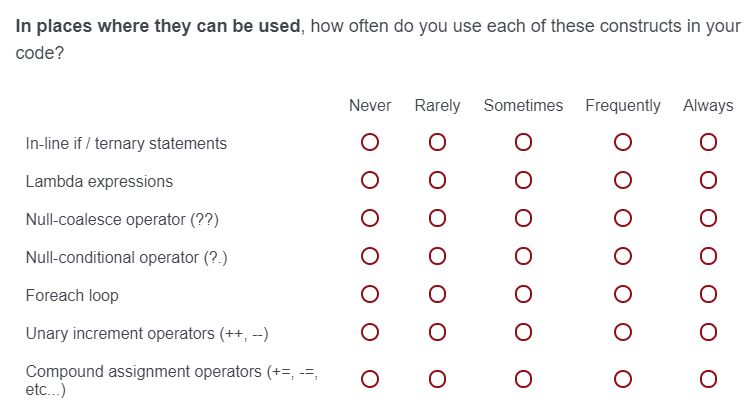
\includegraphics[width=0.8\textwidth]{matrixTable}
            \caption{A matrix table question used in the survey.}
            \label{fig:matrixTable}
        \end{figure}

        \newpage
        \subsubsection{Survey Goals}
        \label{subsubsec:surveyGoal}
            Prior to designing, it was established that the survey must be able to provide insight that may help to answer key research questions. As software development and programming are taught in a multitude of different ways, we can make no assumptions about how familiar participants would be with any of the constructs. To address this, the base questions needed to answer: \emph{What} constructs do they know of? \emph{When} do they use the constructs? \emph{Why} do they use the constructs? From this, some additional, more speculative questions could be asked. The following questions were formulated to best gather as much information as possible:

            \begin{enumerate}
                \item Are the participants \emph{aware} of the constructs?
                \item Do the participants \emph{use} the constructs?
                \item Are participants \emph{encouraged to use} the constructs?
                \item Do the participants think these constructs are better for:
                \begin{enumerate}
                    \item brevity?
                    \item clarity?
                    \item code efficiency/performance?
                \end{enumerate}  
                \item Do the participants think that the constructs are better used in some languages than in others?
                \item Do participants rewrite code either \emph{to use} or \emph{to not use} the constructs?
            \end{enumerate}
            
        \subsubsection{Participants}
            A convenience sample of participating developers was recruited from within the Information Systems Services department (ISS) within Lancaster University by means of a blanket email sent out to all ISS teams and filtered down via regular communications channels within the department. This gathered 40 responses in total, 23 of which completed the survey and may be considered valid responses.
            
            Due to the distribution method, there is no guarantee that all respondents are software developers by profession, however, all participants reported a minimum of one year of programming experience, nearly half falling into the 1-4 years' experience category, with three participants having between 10 and 14 years' experience and the remaining 8 having over 20 years' experience. This statistic was the only personal data collected and does not identify participants.

        \subsubsection{Questions}
            The survey was created using Qualtrics, as provided by Lancaster University, and consisted of a maximum of 16 questions and a minimum of 2 questions (depending on certain answers).
            Participants were first asked to indicate which of the constructs they were aware of so that only questions and options relating to those constructs that they were aware of were shown to them. For each construct they were aware of, participants were asked to answer a series of questions designed to address the questions listed in Section \ref{subsubsec:surveyGoal}, focussing on: frequency of use, reasons to and to not use each construct, perception of effect on code performance, and perception of industry-wide usage per-language.
            
            Lastly, participants were asked if they had any further comments, which invited some very interesting points that will be discussed alongside the rest of the results in Section \ref{subsec:results}.

    \subsection{Static Code Analysis}
        Static code analysis is concerned with checking programs and code for errors without the need to actually execute it. That is, a static code analysis tool will read the source code (or the compiled intermediary language in some cases), construct some form of abstract model of the program and then run a series of tests (often pattern-matching in nature) to detect well-known possible pit-falls, bugs, and problems \citep{staticCodeAnalysis}.

        These tools may make recommendations on how source code may be improved in numerous ways beyond explicit bugs and problems, such as stylistic improvements that make use of advanced syntax whatever given language is being analysed - advanced syntax akin to the constructs being examined here. Accordingly, static analysis tools were employed to investigate whether or not they made any recommendations for or against any of the constructs in question. SonarQube\footnote{https://www.sonarqube.org/} and Semgrep\footnote{https://semgrep.dev/} were selected for this purpose as they both support all three languages being subject to analysis, they are both under recent, active development, and because they both have free variants. Both tools were run against sample control code files and large open source repositories in the earlier mentioned three languages: C\#, JavaScript, and Java.
            
        \subsubsection{Sample Code Files}
        \label{subsubsec:sampleFile}
            Sample code files were created to act as a baseline or control test to see if SonarQube or Semgrep made any note at all about the bare use and/or inclusion of any of the constructs.

            Each file contains a bare (non-contextualised) example of each of the constructs placed directly alongside their `simple syntax' functionally equivalent counterparts. Each file is valid syntax for its language, and all of them may be executed, though none of them have a true entry point or way to actually \emph{run} the code within itself - the functions and methods are present purely to \emph{be present} so that they may be analysed by SonarQube and Semgrep. Though there are differences between the three languages, the form of the sample code was kept as similar as possible to preserve their purpose as control samples, without adding deliberately unusual syntax that may contaminate the output of SonarQube and Semgrep. The sample files can be found in Appendix B.

        \subsubsection{Open Source Repositories}
        \label{subsubsec:osRepos}
            Four large, open source code repositories were selected from GitHub to be analysed for this study, one each in C\# and JavaScript, and two in Java. The selection process was thought to be a random selection from the first page of the most popular GitHub repos for each language, however, it was discovered late in the process that the list from which the repos were selected was actually the `trending today' listing.  Fortunately, the repos that were selected, while potentially not as random or representative as initially thought, are still well known, very active repositories maintained by a diverse range of developers.

            The four analysed repositories are:

            \begin{itemize}
                \item .NET Windows Forms
                \begin{itemize}
                    \item https://github.com/dotnet/winforms
                    \item Commits: 4,339
                    \item `Windows Forms is a .NET Core UI framework for building Windows desktop applications.'
                \end{itemize}
                \item Java Checkstyle
                \begin{itemize}
                    \item https://github.com/checkstyle/checkstyle
                    \item Commits: 10,272
                    \item `Checkstyle is a development tool to help programmers write Java code that adheres to a coding standard. By default it supports the Google Java Style Guide and Sun Code Conventions, but is highly configurable. It can be invoked with an ANT task and a command line program.'
                \end{itemize}
                \item Signal Server
                \begin{itemize}
                    \item https://github.com/signalapp/Signal-Server
                    \item Commits: 1,639
                    \item `Server supporting the Signal Private Messenger applications on Android, Desktop, and iOS'
                \end{itemize}
                \item NPM CLI
                \begin{itemize}
                    \item https://github.com/npm/cli
                    \item Commits: 10,263
                    \item `The package manager for JavaScript'
                \end{itemize}
            \end{itemize}

    \subsection{Git Commit Analysis}
        To supplement the static analysis of the repositories, manual, by-hand analysis of the commits made to these repositories was also undertaken.

        The goal of this branch of the study was to understand if and how standards are being maintained within the repositories with reference to the constructs and to general style-keeping. On a more functional level, the goal was to spot and highlight any cases of code being amended from `plain' syntax to using an advanced construct, or vice-versa. This was carried out by cloning the repository and examining the commit history. Due to the sheer number of total commits available in the selected repos (approx. 26,500), it would be unfeasible to check every commit for every relevant kind of change in the timescale of this study. To overcome this, a list of keywords was run against the commit history to filter results using the \codeword{--grep=<pattern>} option to \codeword{git log}. The keywords used are listed in Table \ref{tab:keywords}:
        
        %\begin{center}
        \begin{table}[ht]
            \centering
            \begin{tabular}{ | l | l | }
                \hline
                \textbf{General} & style \\
                \hline
                \textbf{Ternary} & ternary, conditional, \codeword{?:} \\
                \hline
                \textbf{Null coalesce/conditional} & null, coalesce, conditional, \codeword{??}, \codeword{?.}, \codeword{?[} \\
                \hline
                \textbf{Lambda} & lambda, arrow, \codeword{=>}, \codeword{->} \\
                \hline
                \textbf{For each} & foreach, for each \\
                \hline
                \textbf{Unary Operators} & unary, increment, decrement, ++, -{}- \\
                \hline
                \textbf{Compound Operators} & compound, assign, \codeword{+=}, \codeword{-=}, \codeword{*=}, \codeword{/=}, \codeword{|=}, \codeword{&=} \\
                \hline
            \end{tabular}
            \caption{Keywords used in manual analysis of repository commit messages.\label{tab:keywords}}
            
        \end{table}
        %\end{center}

        Some of these keywords generated cross-over between those meant to highlight changes around a particular construct, but this was unimportant as these keywords were only used to create a list of  `interesting' commits. Commits were deemed interesting if the commit message and/or description contained reference to any of the keywords in such a way that it seem plausible that a change was made regarding any relevant construct. For each commit in the resultant list, the changes were scrutinised closely to pick out changes made that: added, removed, altered, or commented on use of any of the constructs. Each type of change was documented and counted per commit.

        After analysis was complete, my subjective classification was validated by use of a second rater. This rater was provided with 10\% of the interesting commits and was asked to pick out any changes they could identify in these commits and to classify them as a change pertaining to one of the constructs, and whether it was a change to add or remove the construct. From the second rater's classifications, agreement was calculated using Cohen's Kappa, giving a kappa value of \codeword{ k = 0.99}. According to \cite{cohensKappa}, this equates to an `almost perfect' agreement, and is more the high enough to proceed with analysis based on my classification.

    \subsection{Intermediate Language Comparison}
        The final part of this study was brought about during the progress of the preceding work. Analysis of the survey results raised some interesting points and potential ideas around what may make certain constructs more or less suited to use generally, and in any given place in code.

        C\# and Java, while both are compiled languages, they are compiled to an intermediate language which is then interpreted by a virtual machine for execution. This means that we may examine the intermediate language (IL) to understand if there are any clear differences between the plain and advanced forms of syntax and constructs. This would be a somewhat crude way to go about attempting to gauge the difference in performance or efficiency, but merely examining and commenting on the difference in C\# and Java's respective ILs can prove valuable as supporting material to this study.
        
        The code files used to generate the IL code contained the same code as in the sample files mentioned in Section \ref{subsubsec:sampleFile} with one change: the sample code files have consecutive functions, one in plain syntax, one using an advance construct. To make analysis and comparison easier, the plain and advanced syntax functions were extracted into separate files so that there was a plain syntax \emph{file} and an advanced syntax \emph{file}. This allowed ease of comparison using git integrations with Visual Studio Code to perform a \codeword{git diff} to see the similarities and differences easily. 

        For C\#, the online tool SharpLab \footnote{https://sharplab.io/} was used to produce .NET Common Intermediate Language using Microsoft's Roslyn  compiler. For Java, `JVM Bytecode Viewer' for Visual Studio Code \footnote{https://marketplace.visualstudio.com/items?itemName=mnxn.jvm-bytecode-viewer} was used to locally open the .class files produced by the JDK to view the code.

\newpage
\section{Results}
    \subsection{Survey}
    \label{subsec:results}
        As described in Section \ref{subsec:survey}, a survey was conducted with experienced software developers and programmers. This revealed interesting patterns of usage (or lack of usage) of the constructs, and some interesting perceptions that may prove useful in future research focussed on performance and use in the wider industry.

        The following sections will detail the results of the survey, followed up by a note on the threats to the usefulness of, and the patterns discovered by the survey. All percentage values given in text have been rounded to one decimal place unless otherwise stated.

        \subsubsection{Awareness}
            Awareness of the constructs was gathered by a simple multiple-choice question with a binary yes/no for each. Participants could indicate whether or not were familiar with all, some, or none of the constructs.
            \\\newline
            All participants were aware of unary operators and ternary/in-line if-statements, nearly all were aware of compound operators and lambdas, and most were aware of null-coalesce and null-conditional. Figure \ref{fig:awareness} shows these results in a graphic format.

            \begin{figure}[htbp]
                \centering
                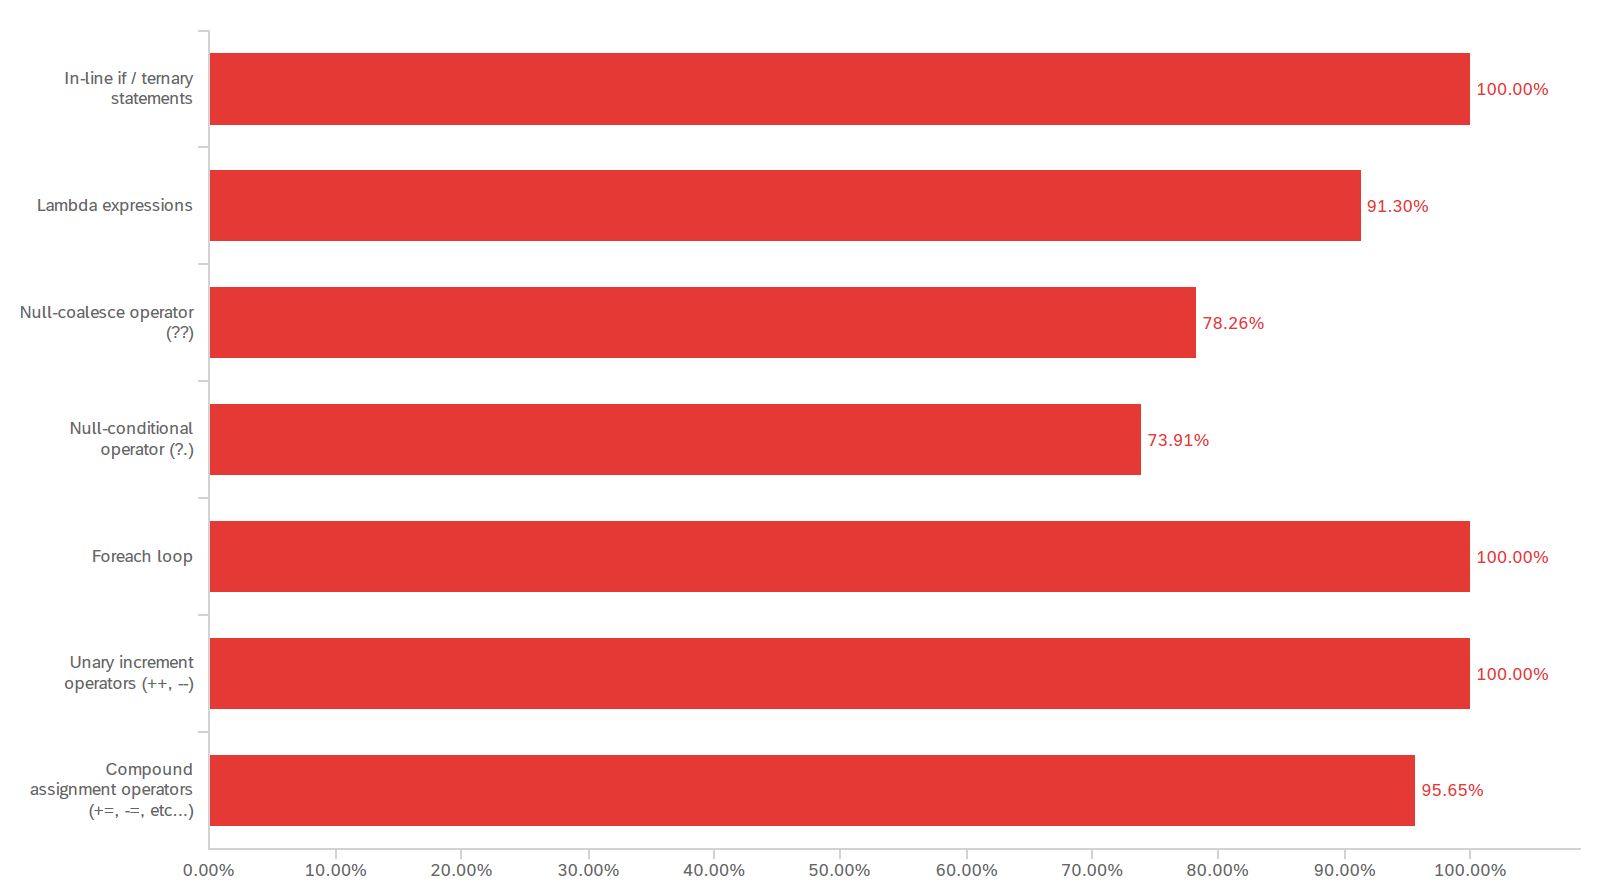
\includegraphics[width=1.0\textwidth]{awareness}
                \caption{Percentage of participants aware of each construct}
                \label{fig:awareness}
            \end{figure}

            The most stand-out piece of information here is that the awareness of the null-coalesce and -conditional operators was markedly higher than might be expected due to the relatively lower availability of these operators. This can likely be attributed to the fact that participants were all from within ISS, where the  technology stack contains a large amount of C\#, in which these operators are often seen. If the survey were repeated over a more diverse and broad range of developers working in more varied technology stacks (for example, those focussed much more on Java, or C/C++), it is reasonable to assume that awareness of these operators would be diminished. This is a trend that is repeated elsewhere in the results set.
            It is also of note that not \emph{all} participants were aware of compound assignment operators, whereas all participants \emph{were} aware of ternaries - a ranking inverse to what was expected. However, the difference in the numbers is not very large, comprising no more than one or two responses. To draw any valid conclusion from this datum would require it being replicated in a greater sample set.

        \subsubsection{Frequency of Use}
            To assess how often participants use each of the constructs, they were asked specifically: \textit{In places where they \textbf{can} be used, how often do you use each of these constructs in your code?}, that is taken to mean:, ``for every chance you \emph{could} use the construct, how often do you use it?''
            \\\newline
            It was the extreme ends of the scales in this question that provided the most interesting results here. Firstly, only one data point was recorded for any construct under the `never' option, with just one respondent indicating that they never use the null-coalesce operator. This is perhaps reassuring given that it's generally accepted that most of these constructs have at least \emph{some} place to be used. Conversely, `for each' was the most selected construct in the `always' category, with 43.5\% of participants selecting this option, followed closely by compound assignment operators at 40.9\%.

            Across all constructs, the majority of responses fell into the `frequently' category, holding 39.5\% of the total selections, with the `sometimes' category at 27.2\%. This general erring toward the more frequent end of the scale holds not only for the collective dataset but also for each construct when examined individually, as may be seen in figure \ref{fig:freqUse}.

            \begin{figure}[htbp]
                \centering
                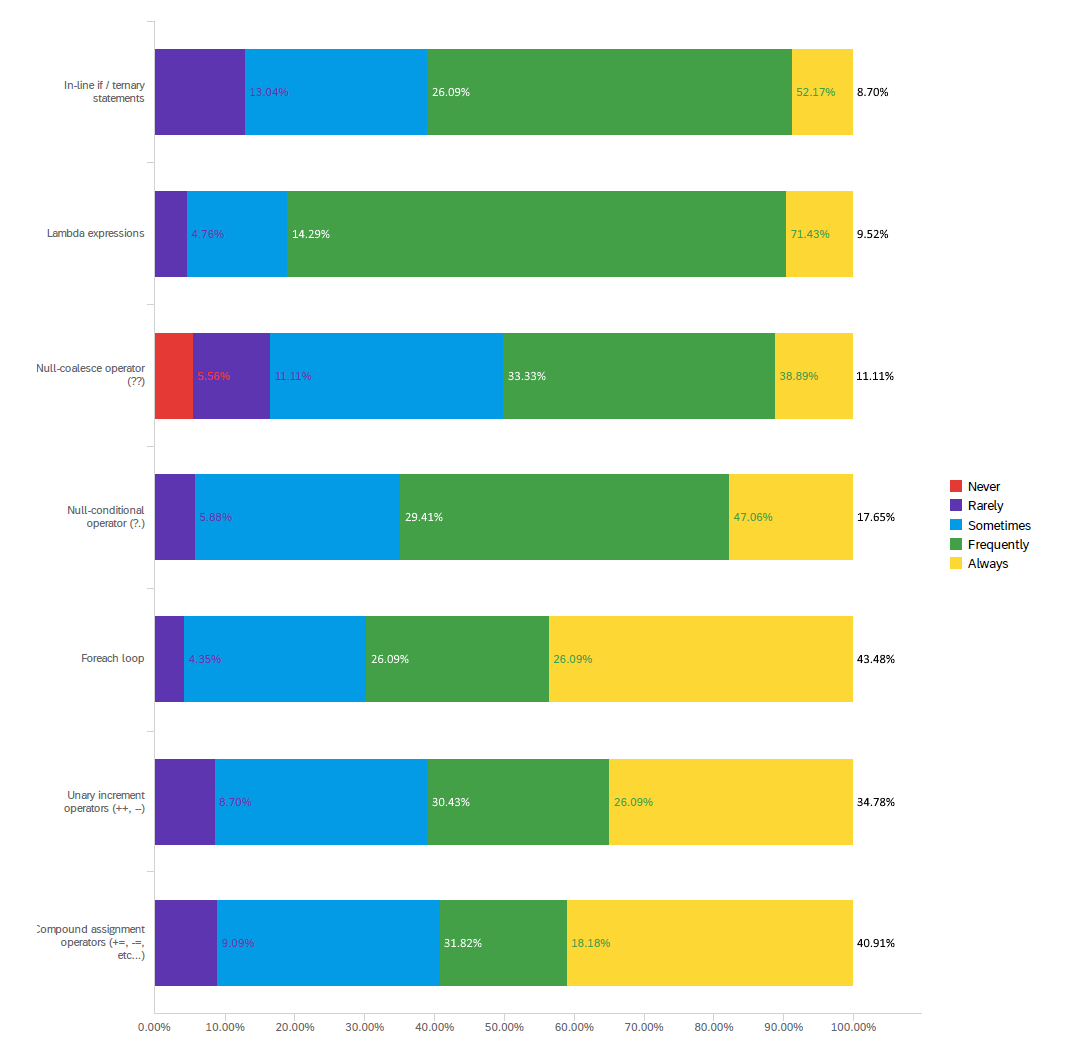
\includegraphics[width=0.9\textwidth]{freqUse}
                \caption{Frequency with which participants said they used advanced constructs, grouped by construct. (n.b. figures normalised to percentages)}
                \label{fig:freqUse}
            \end{figure}

            As is visible in Figure \ref{fig:freqUse}, the use of lambdas often but in moderation is the most agreed upon data point here, with 71.4\% of responses labelled `frequently' for lambdas. This is likely explained by a variety of reasons, not least being the fact that lambdas are very powerful and complex structures, much more so than the other constructs being studied, and as such, the number of situations where they \emph{can} be used likely greatly exceeds the number situations where they \emph{should} be used. This distinction around lambdas becomes more apparent in later questions.
            Of note, again, are the results for the null-coalesce and null-conditional operators. Although the numbers of participants familiar with these operators is fewer, those that were aware of them do not shy away from them, using them with comparatively similar frequency to the other constructs.

        \subsubsection{Reasons To Use}
        \label{subsubsec:toUse}
            Participants were then asked to indicate \emph{why} they chose to use each given construct. The four options presented were:
            \begin{itemize}
                \item ``It is company style''
                \item ``It makes code clearer''
                \item ``It makes codes simpler''
                \item ``It makes code run faster''
            \end{itemize}
            One or more of the above options may have been selected, with an additional exclusive option: ``None of these'' present too. If this was selected, participants were prompted to give their own reason in the following question.
            \newline

            The trend here was extremely clear: the most common reasons for using any of the constructs were for clarity and simplicity. ``It makes code clearer'' and ``It makes code simpler'' took 39.4\% and 42.3\% of \emph{all} selections made respectively. The data for the selections totalled across each construct is shown in Figure \ref{fig:toUse}a.

            Six participants selected `None of these' for at least one construct, two of whom selected this option for all constructs they were aware of and both instead said that they choose to use the constructs based on personal preference or habit. Another two selected this option for lambdas alone, one saying that they are aware of, but don't use lambdas, and the other highlighting a possible flaw in this study regarding lambdas. This participant noted that there are places where ``there is no rational alternative to using a lambda expression. It does not make the code simpler or clearer, it's just \textbf{necessary} to use a lambda.'' This brought to attention the fact that lambdas may be a more functional language feature, not fitting in the same category as the other constructs here, which can mostly be categorised as `syntactic sugar' that do not have much actual difference on code functionality. This is discussed further in Section \ref{subsubsec:lambdas}.
            One participant also said that they would generally use `map' instead of a foreach loop. `Map' is presumably referring to the \codeword{map()} function in JavaScript that may be called on an array to perform a function on all elements of the array - the function to apply is taken by \codeword{map()} as an argument, either via lambda or regular method or function. They claim using \codeword{map()} ``helps avoid `off by one' errors''.  Off-by-one-errors occur when iterating over an array or other list of \textit{m} through \textit{n} items and having the index incorrect by one. For example, if you were to ask how many items there are (how many loop iterations are required) in a collection of items, the intuitive answer of \textit{m} - \textit{n} is incorrect, the correct answer being (\textit{m} - \textit{n}) + 1. This is illustrated in Figure \ref{fig:fencepost} using a specific type of off-by-one error, a \textit{fencepost error}.
            \\

            \begin{figure}[htbp]
                \centering
                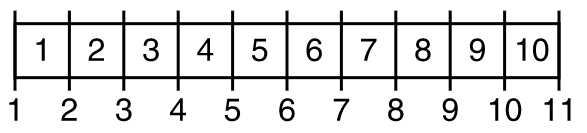
\includegraphics[width=0.5\textwidth]{fencepost}
                \caption{If you have a straight fence 10 meters long, with posts spaced 1 meter apart, how many posts are present? An intuitive answer may be 10, but it is in fact 11. This is a specific off-by-one error.}
                \label{fig:fencepost}
            \end{figure}

            It is not clear what advantages a `map' function has over a foreach loop to avoid off-by-one errors. In fact, conventional wisdom dictates that foreach loops, by nature should, avoid these errors by virtue of the fact that they \emph{remove} the need for a programmer to calculate the necessary number of loop iterations or use an index at all. It is plausible to suggest that this response was given by mistake, instead meaning to refer to traditional for loops, rather than foreach loops.

            Figure \ref{fig:toUse}b part repeats the data in \ref{fig:toUse}a, again showing that clarity and simplicity are the most common reasons. We can also see that the split is \emph{mostly} even between these two reasons, null-coalesce being a slight exception, with nearly double as many responses selecting simplicity over clarity. Null-conditional follows this pattern, but the difference is less pronounced.
            Other notable statistics are: no participants said that they used null-coalesce or -conditional due to company style, and the three constructs that had code run speed selected. Two participants selected this for lambdas, and one each both selected this for foreach loops and unary operators. These selections do not represent a large proportion of the total, but it is still of note that none of the other constructs had any selections regarding faster code execution.
            
            \begin{figure}[htbp]
                \centering
                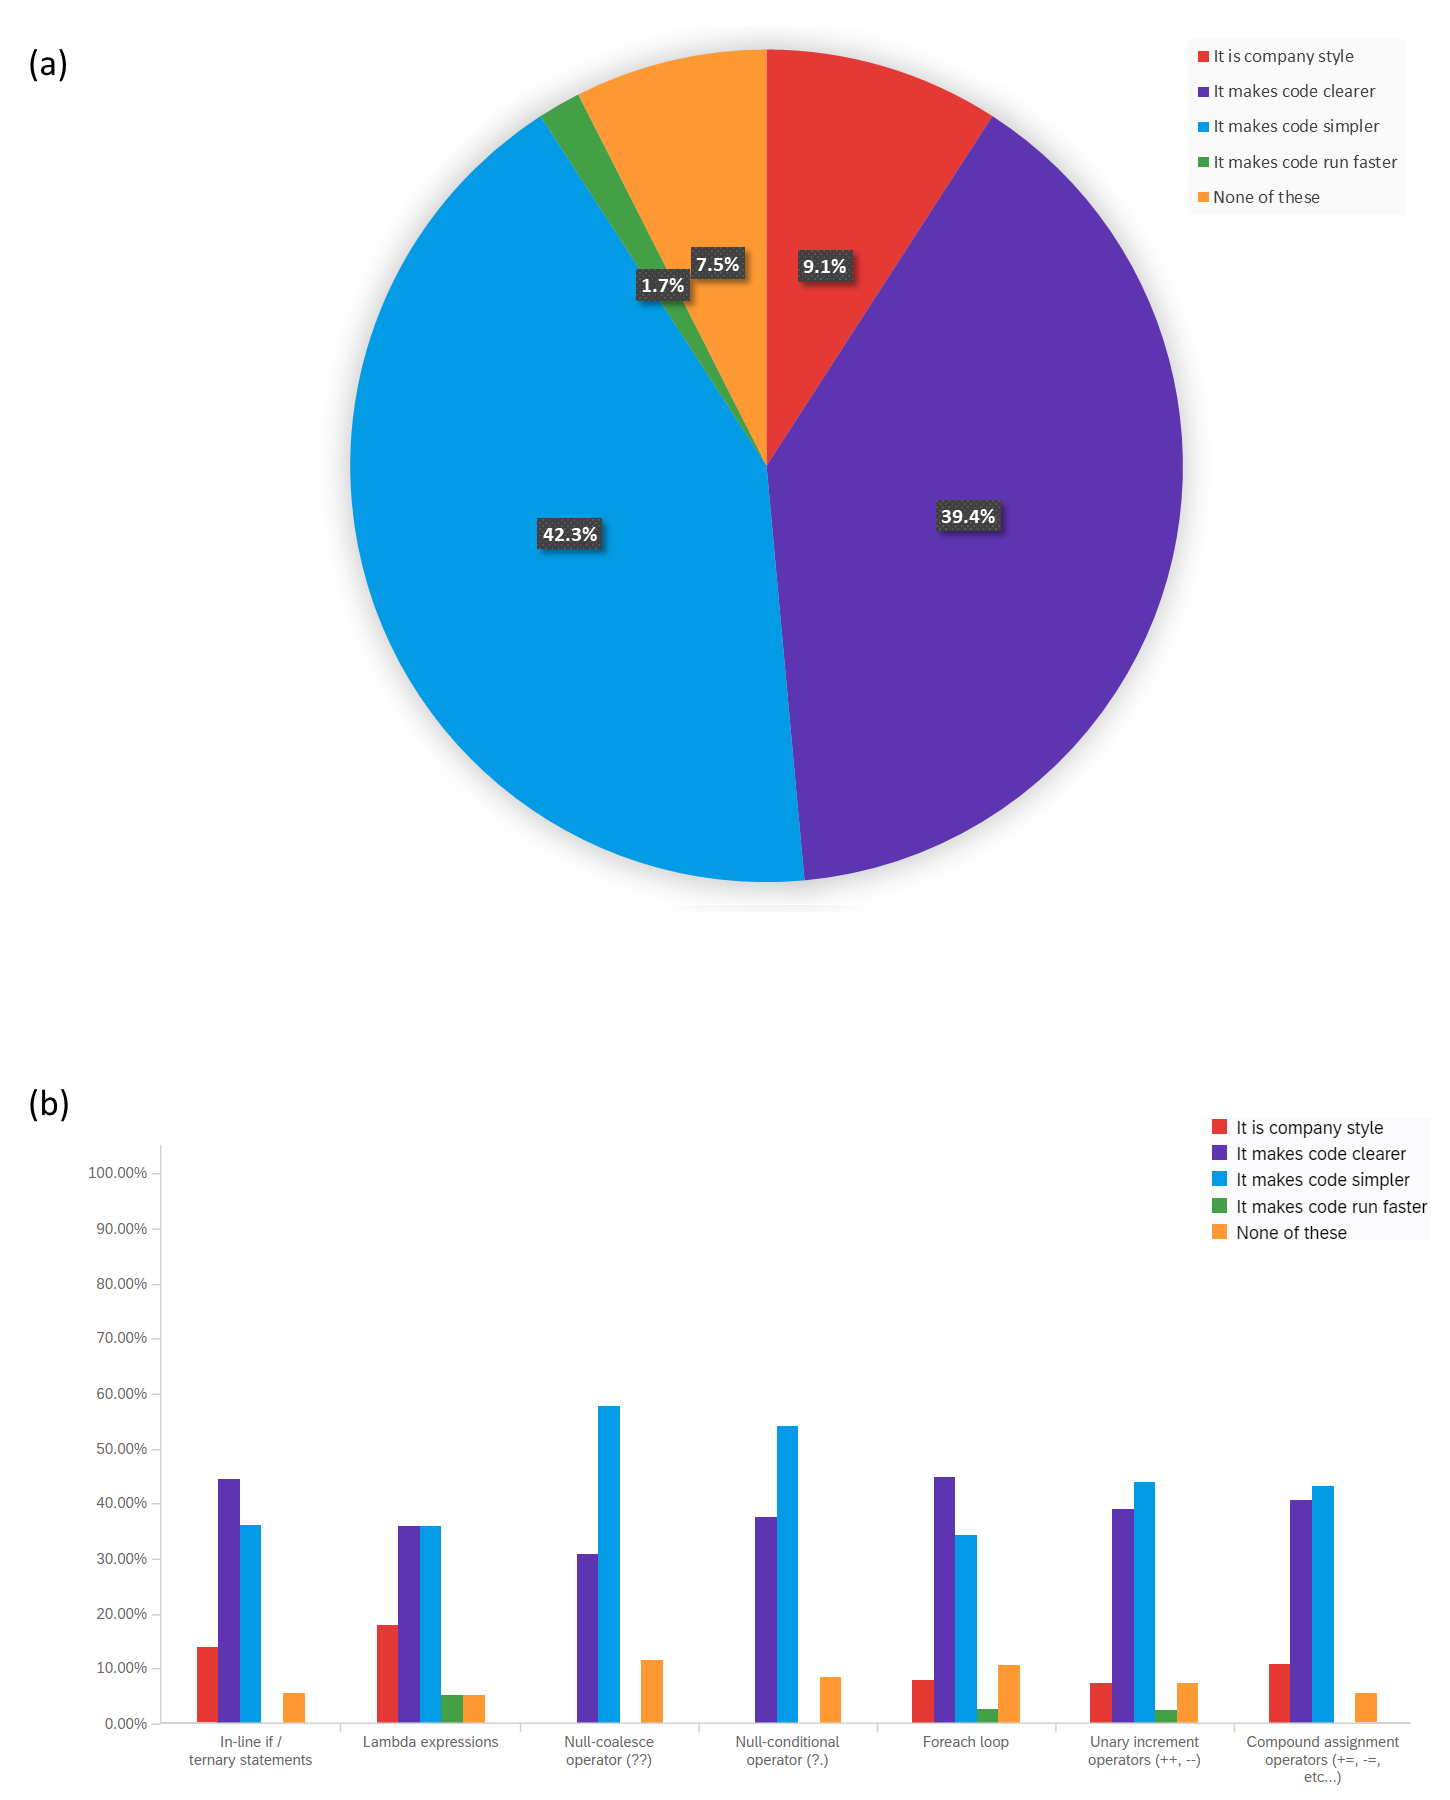
\includegraphics[width=0.9\textwidth]{toUse}
                \caption{(a). Reasons to use constructs, totalled across all constructs.\newline (b). Reasons to use constructs grouped by construct. (n.b. Figures normalised to percentages per construct)}
                \label{fig:toUse}
            \end{figure}

        \newpage
        \subsubsection{Reasons To Not Use}
            To provide the other half of the story to the previous section, participants were also asked about the reasons they choose to \emph{not} use the constructs. Similar to before, the options presented were:
            \begin{itemize}
                \item ``It is company style''
                \item ``It would make code less clear''
                \item ``It would make code more complex''
                \item ``It would make code run slower''
            \end{itemize}
            As before, one or more of the above options may have been selected, with a ``None of these'' option that prompted participants to give their own reason(s) if selected.
            \newline

            Reasons of clarity and complexity were the most selected again, with 48.2\% of all selections attributing maintenance of clarity as a reason to not use a given construct, and complexity at 23.9\%. More than double the proportion of selections were present for ``None of these'' compared to when asked for reason \emph{to} use the constructs - here, 16.2\% of selections were ``None of these''. The reasons provided by these respondents were quite varied but very interesting and are all worthy of discussion:

            \begin{itemize}
                \item Personal preference
                \begin{itemize}
                    \item Mentioned explicitly by three, and implicitly by one, of the ten individuals who gave their own reasons.
                    \item One noted that ``as long as code is well documented you can use any of them''.
                    \item One wrote that there is no company style for these constructs and that there is instead guidance on larger/less granular things like examples of a model class. This is contradicted by other responses (which occasionally imply that there \emph{is} a company style), though it's plausible they are subject to different coding standards within ISS.
                    \item The third, the only of the ten that overlap with those that selected this option on the previous question. Simply stating that it is personal preference.
                    \item The final respondent's reason links the usage of compound and unary operators going against their preference to use a `functional style' and to `avoid mutability of variables'. This raises interesting questions about the use of functional programming ideas in non-functional paradigms.
                \end{itemize}
                \item `I [almost] always use this construct'
                \begin{itemize}
                    \item Two participants said they would always use unary increment operators.
                    \item One said they would always use compound operators.
                    \item Another said the only time there would not use null-coalesce/null-conditional is when null checking is not required at all.
                \end{itemize}
                \item Other/Unqualified
                \begin{itemize}
                    \item One participant stated that a for loop may be preferable to a foreach loop when the index variable is needed. They then go on to say that it also `depends how I'm feeling'.
                    \item Regarding lambdas and unary and compound operators, one participant said: ``sometimes these operators don't account for requirements such as type checking or formatting'' without any more description.
                    \item One participant claimed that foreach loops may introduce errors but did not explain further.
                \end{itemize}
            \end{itemize}

            \begin{figure}[htbp]
                \centering
                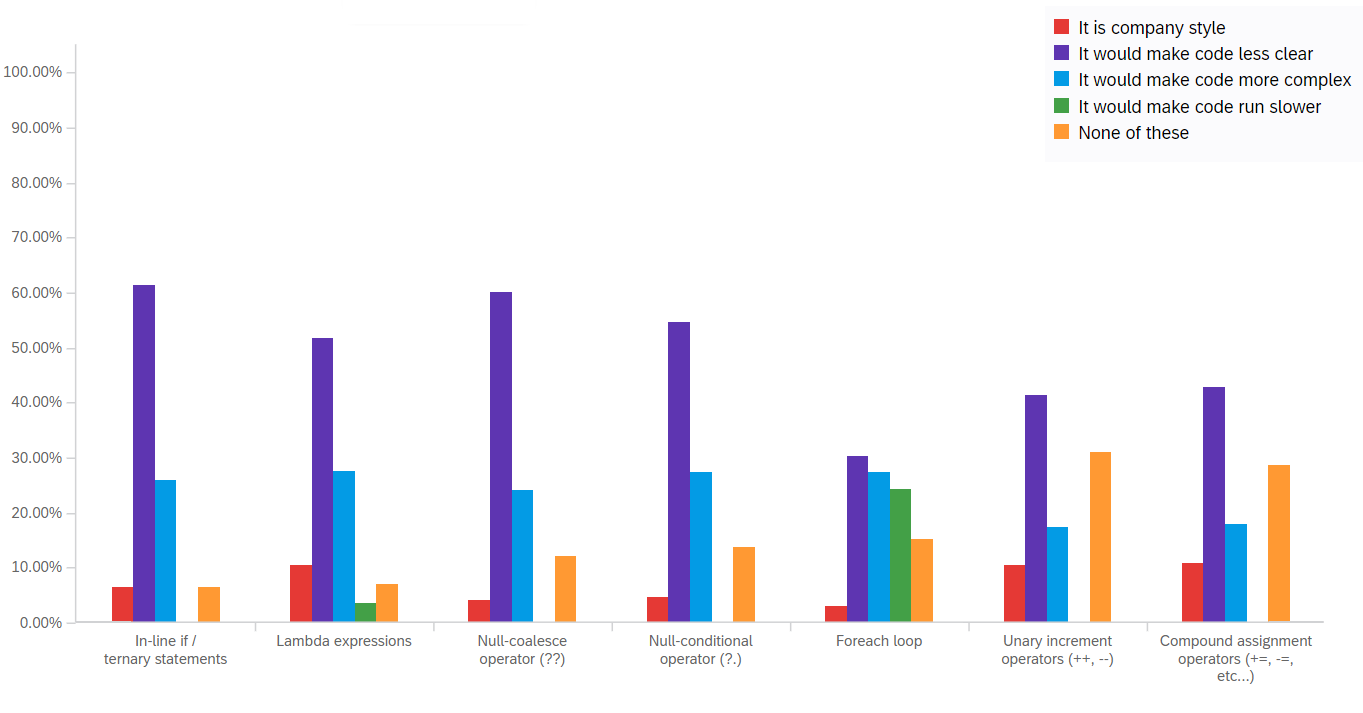
\includegraphics[width=0.9\textwidth]{toNotUse}
                \caption{(a). Reasons to not use constructs, totalled across all constructs.\newline (b). Reasons to not use constructs grouped by construct. (n.b. Figures normalised to percentages per construct)}
                \label{fig:toNotUse}
            \end{figure}

            Only 4.5\% selected ``It would make code run slower'' - logically, this would make sense as it generally assumed that most of these constructs are plain syntactic differences that, with most modern compilers and interpreters, may produce the same bytecode and/or machine code. This is however disproven later in Section \ref{subsec:ilComp}, but participants may not have known otherwise at the time. Lambdas and foreach loops are likely the only exceptions to this. The former has other potential implications beyond just how it looks on-screen, the latter (depending on language) may be a change from an array index to initialising an iterator and calling on that instead. This is reflected in the thoughts of participants in Figure \ref{fig:toNotUse}b, showing that these two constructs were the only two to have received any selections pertaining to code run speed.

            The breakdown in Figure \ref{fig:toNotUse}a also confirms that clarity was the most common reason selected, leading by a wide margin for four of the constructs, but not for unary and compound operators (due to multiple reasons, described above) and for foreach loops (run speed was a concern as described immediately above).
            All constructs had a small number of responses claiming company style as reasons for not using them, but this is a relatively small number compared to the proportion that cited clarity or complexity.

        \subsubsection{Performance}
            As touched on previously, it was not expected with most of these constructs for there to be much of a bias with regard to performance (this is examined crudely in Section \ref{subsec:ilComp}). Participants were asked to state what, if any, effect they thought each construct would have on the performance of code.
            \newline

            In line with expectation, a majority, 61.2\%, of the selections here indicated no change to performance. The second largest group was ``Don't know'' with 22.4\% of selections. Both these statistics are shown in Figure \ref{fig:performance}b. It is likely that most high-level programmers (such as those using high-level languages like C\#, JavaScript, and Java) either do not routinely give much consideration to such fine-grained efficiency, or are not concerned with relatively small performance variations that come from using these constructs.

            The individual performance data also matches participants' selections from the previous question when grouped by construct: the majority for each is still ``No change'', but the stand out constructs that have a high number of selections of increased or decreased performance are lambda expressions and foreach loops. Lambdas had the smallest proportion of selections for ``No change'', and the largest for ``Increased performance'', meanwhile foreach had the second smallest proportion of ``No change'' and the largest for ``Decreased performance''. The possible decrease in performance using foreach was discussed in the previous section.

            \begin{figure}[htbp]
                \centering
                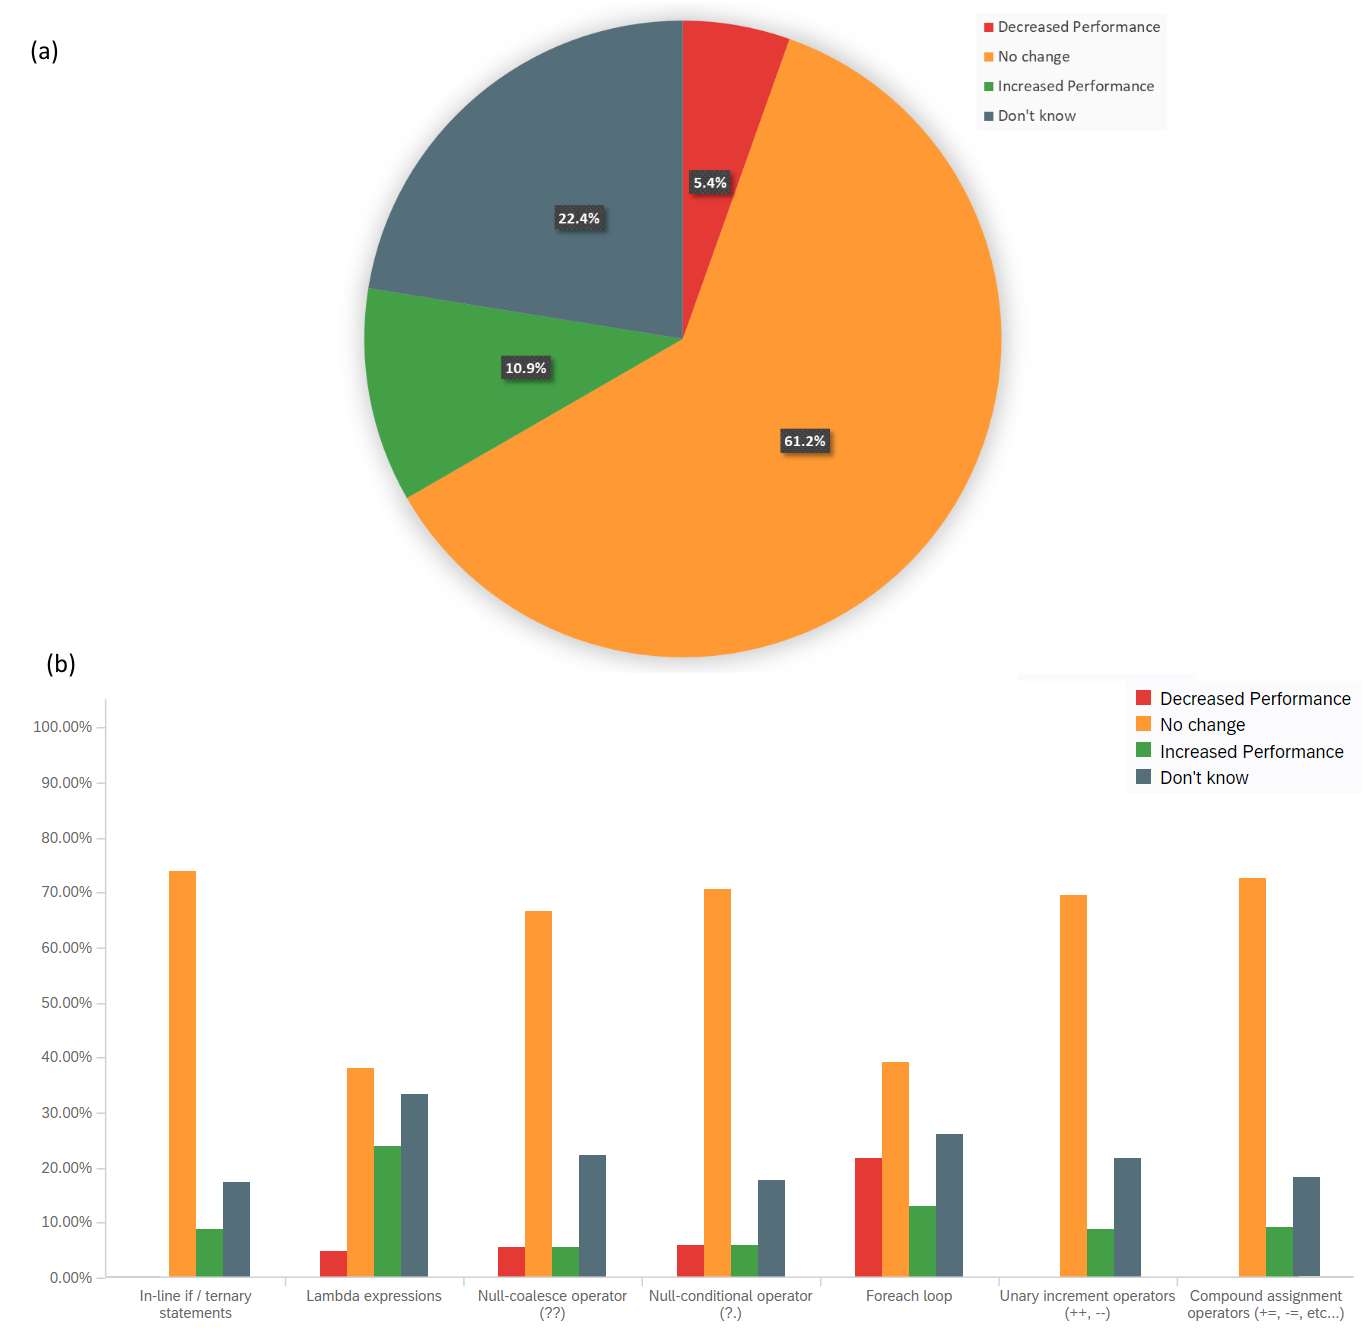
\includegraphics[width=0.8\textwidth]{performance}
                \caption{(a). Selections for performance, totalled across all constructs.\newline(b). Performance selections grouped by construct. (n.b. Figures normalised to percentages per construct)}
                \label{fig:performance}
            \end{figure}   

        \newpage
        \subsubsection{Usage In Wider Industry}
            The final set of questions asked participants about their perception of the prevalence of the constructs in the wider industry of software development, asking whether they thought that use of each construct was above, on par, or below average in any of the three languages when compared with use across the industry in general. Figures \ref{fig:industry} and \ref{fig:industryExcl} collate results across all constructs for this question set, the former including and the latter excluding `Don't know' selections for clarity.

            \begin{figure}[htbp]
                \centering
                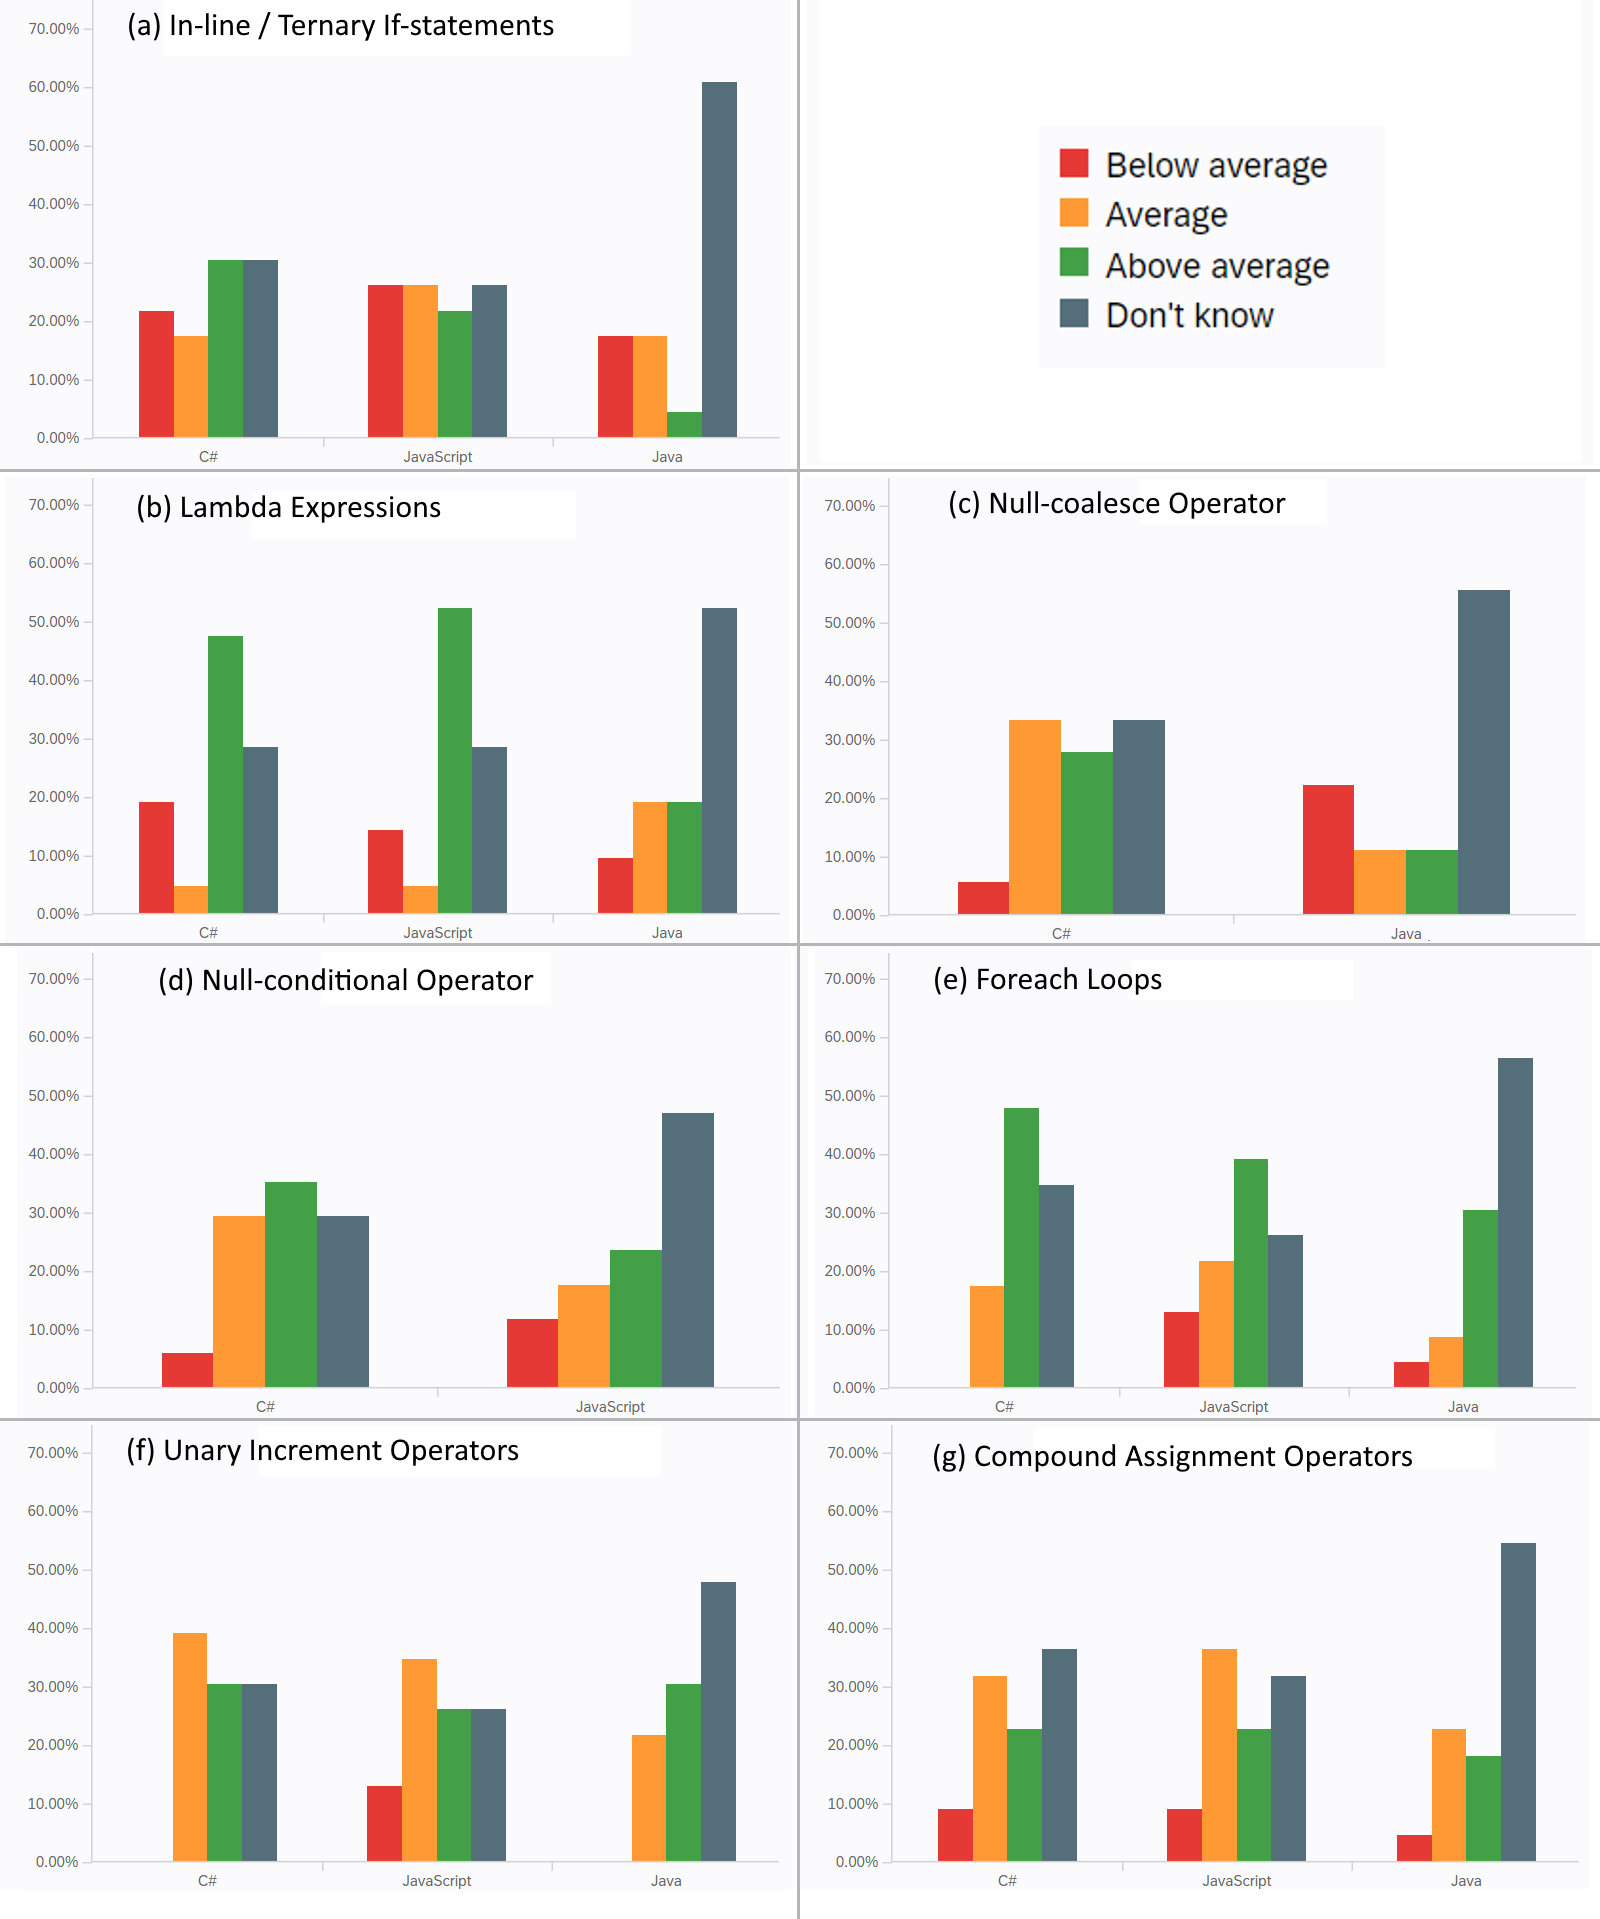
\includegraphics[width=0.9\textwidth]{industry.png}
                \caption{Responses on prevalence in wider industry compared to each language, displayed per construct. A typographical error meant that participants were asked about null-coalesce in Java: this should have been JavaScript, as Java has no null-coalesce operator. That portion of the results should be ignored. (n.b. Figures normalised to percentages and truncated scale, Null-coalesce and null-conditional operators are not present in Java, giving only two groupings)}
                \label{fig:industry}
            \end{figure}

            \begin{figure}[htbp]
                \centering
                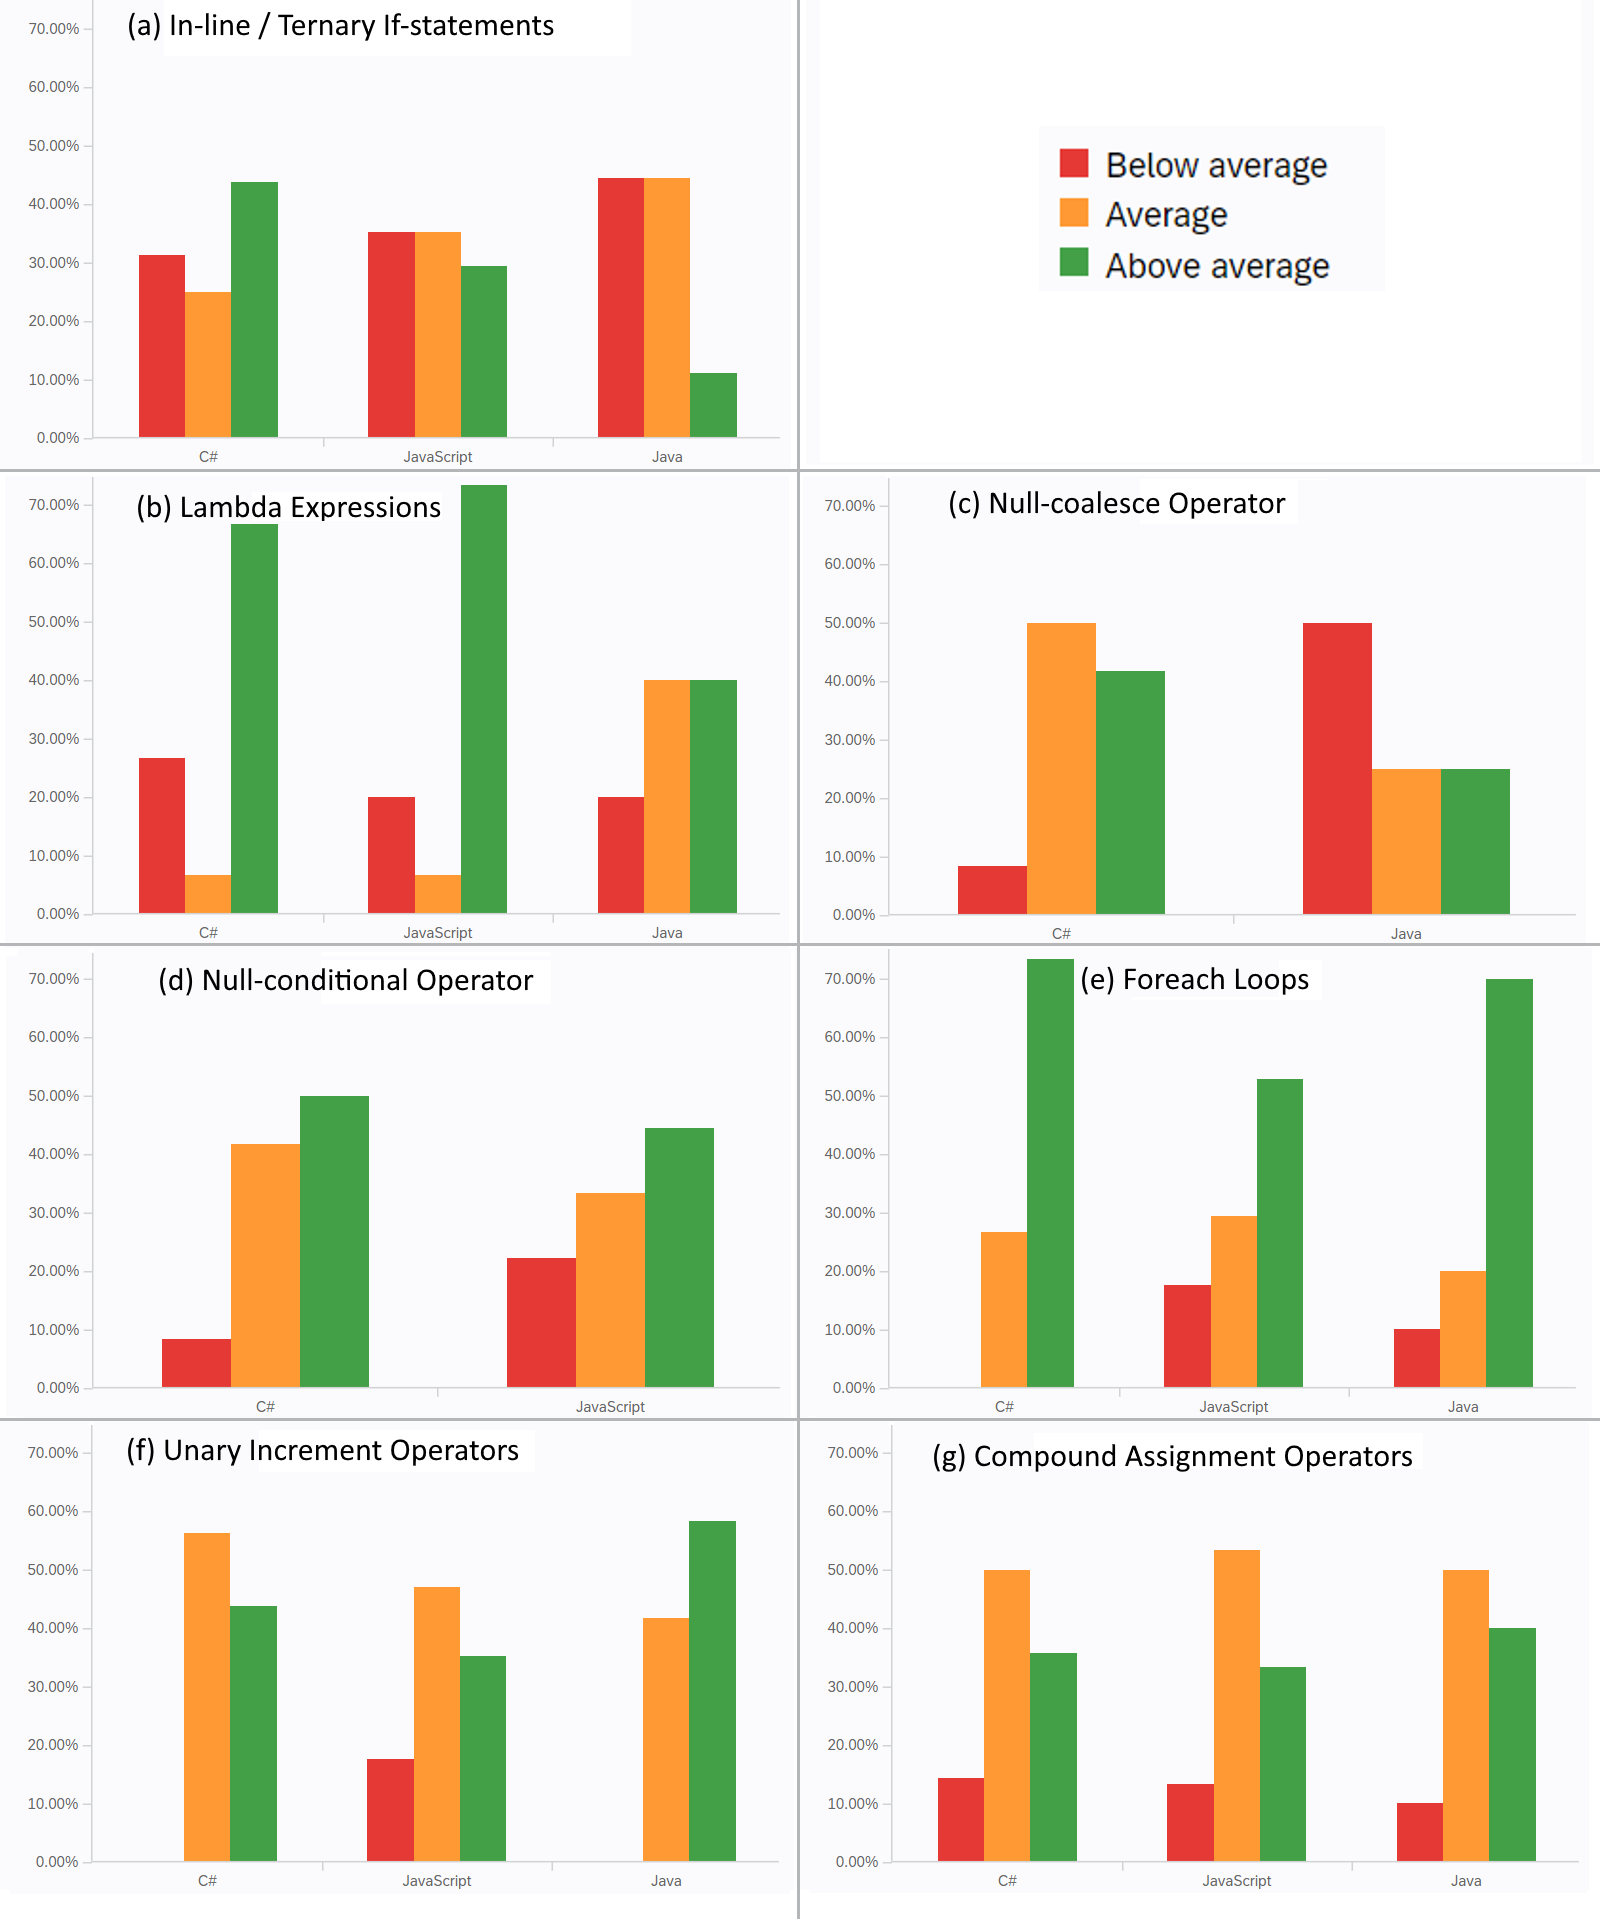
\includegraphics[width=0.9\textwidth]{industryExcl}
                \caption{The same as Figure \ref{fig:industry}, but excluding ``Don't know'' responses.}
                \label{fig:industryExcl}
            \end{figure}

            In general, responses were quite scattered, and the most clearly discernible patterns are centred on the ``Don't know'' responses.

            The most consistent pattern across the entire set of responses was that of uncertainty around usage of the constructs in Java. This will likely be due to the fact that ISS does not use Java in its tech stack anywhere. The most obvious case of this is for ternary if-statements, with 60.9\% of all responses for Java being ``Don't know''. Also, lambda expressions and foreach loops were perceived as being more common in C\# and JavaScript by a majority.

            The following breakdown summarises results for each construct, excluding ``Don't know'' responses from figures:
            
            \begin{itemize}
                \item In-line if / Ternary If-Statements
                \begin{itemize}
                    \item Received the largest number proportion of ``Below average'' selections for any language or construct, the other selections were also high giving a mean value corresponding to just marginally \emph{above} average for C\#, marginally \emph{below} average for JavaScript and just above the midpoint between below average and average for Java.
                \end{itemize}
                \item Lambda Expressions
                \begin{itemize}
                    \item At least one of each selection, but with ``Above average'' outstanding for C\#, and particularly so for JavaScript. C\# and JavaScript have a mean corresponding to just midway between average and above average, and Java a little above average
                \end{itemize}
                \item Null-coalesce
                \begin{itemize}
                    \item The mean for C\# gives a value a little above average, while, as mentioned above, a typographic error means no data was collected for JavaScript and the Java data is unusable.
                \end{itemize}
                \item Null-conditional
                \begin{itemize}
                    \item Both trend toward average/above average, with C\# having a mean lying at the midpoint between average and above average and JavaScript lying a little above average.
                \end{itemize}
                \item Foreach Loops
                \begin{itemize}
                    \item Alongside lambdas, the only other construct strongly perceived as ``Above average''. The mean values for C\# and Java are strongly toward above average while JavaScript has a mean just a little above average.
                \end{itemize}
                \item Unary Increment Operators
                \begin{itemize}
                    \item Means were above average for all languages: C\# midway between average and above average, JavaScript marginally above, and Java strongly above average.                
                \end{itemize}
                \item Compound Assignment Operators
                \begin{itemize}
                    \item Means were again above average for all languages, a little above average for all three.  
                \end{itemize}
            \end{itemize}

            \begin{figure}[htbp]
                \centering
                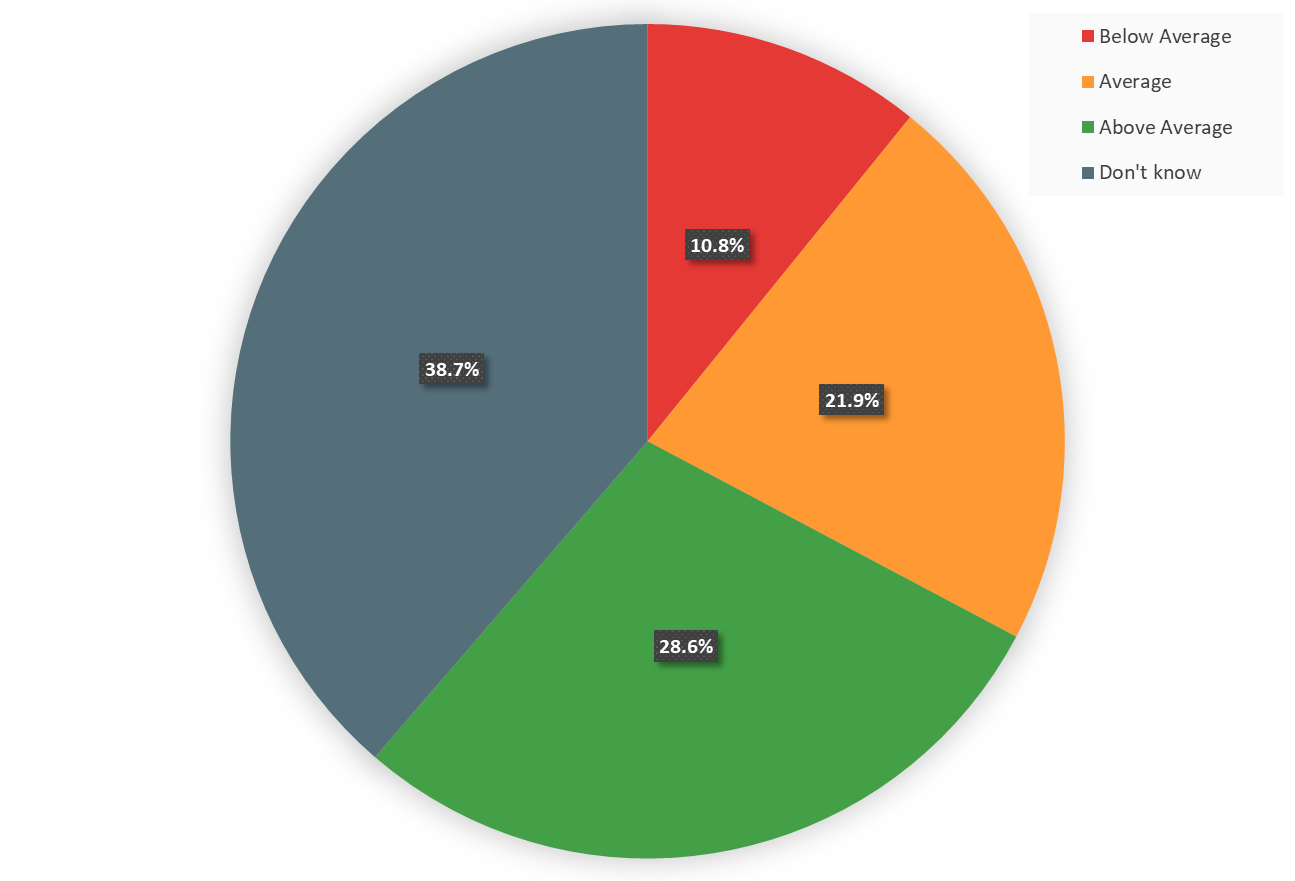
\includegraphics[width=0.9\textwidth]{industryPie.png}
                \caption{Responses on prevalence in wider industry compared to each language, totalled across all constructs and languages.}
                \label{fig:indsutryPie}
            \end{figure}            

        \subsubsection{Free-form Comments}
        \label{subsubsec:freeFormComments}
            The final question asked participants to indicate any other thoughts and notes they had around the topic at hand. This yielded some very interesting comments.

            As has been mentioned already, most of these constructs come under the umbrella of `syntactic sugar' - that which is meaningful only to a human developer and functions the same as their simpler counterparts at machine level. One participant noted this themselves, and further stated that these constructs should be used to save space and time, so long as code readability is not compromised. One more nuanced response gave much more detail, opening with a phrase that sums up the very issue of knowing when to use the constructs: ``Most of these questions [...] are more properly answered `As appropriate''', going on to say that runtime performance ought to be measured only in context, not in isolation. They apply this statement both across different scenarios in the same language and across different languages. They also highlight that in the present day ``we're waiting for [input/output] from the disk or network - the time spent executing each one of those constructs pales in comparison''. The same comment again reaffirms that `everything depends on circumstances', such as in safety-critical systems where code understandability and correctness are of ultimate importance. In such situations, it may be advisable to only use basic syntax and work around that as an axiom, but then again, it may not - proving the point that the context and situation may be one of the most important factors in usage of these advanced constructs, and may also go some way toward explaining why there seems to be little explicit guidance on this matter.

            Another comment stated again that the constructs being examined are syntactic sugar, however, this was written in a way that implied something to the effect ``they are just syntactic sugar and so they don't really matter''. This may not have been the case, but it would be further explanation as how uncertain the situation appears to be around when and how to use such constructs. The same comment separates lambdas out as not syntactic sugar, but a structure that permits more functional practices that can ``fundamentally change how your system is built and hence how it is compiler optimised''. This is one of the pieces of information gathered during the process that has quite clearly marked out lambdas as not quite fitting into the same category as the rest of the constructs (see \ref{subsubsec:lambdas}).

            Lastly, one participant notes that there are times when some of these constructs simply cannot be used, giving the example of writing entity framework expressions in C\# using LINQ. It is perhaps up for debate if LINQ counts as C\# on more than technicality, but it is a valid point that there are places where certain syntax cannot be written or where available syntax is otherwise limited. However, these situations are an edge-case, and are such an edge-case that, should standardised documents be written to define how to use the constructs, it could easily make exceptions for such situations.

        \subsubsection{Threats to Survey}
            The group of survey participants was comprised of a convenience sample of developers from within ISS. This means that the results may not generalise very well to a wider group of developers. The results may be generalised \emph{within} ISS but not outside. Further research and more significant surveying should be undertaken to verify if the results found within ISS may be applied to a wider populace of developers.

            Despite this, a survey still provided a very quick and efficient way to gather information from a sample size much larger than would be feasible using many other methods.

    \subsection{Static Code Analysis}
        SonarQube and Semgrep are both static code analysis tools that analyse code to make recommendations and highlight problems without actually executing the code itself. Both of these tools were used to analyse both the sample code files (see Appendix B) and the four GitHub repos. For C\#, SonarScanner for .NET was used as well as the developmental Semgrep ruleset for C\#. For JavaScript and Java, both were supported by Semgrep rules sets `ci' and `r2c-ci', and both had their own eponymous rulesets too. Standard SonarQube also supports both languages as standard.

        \subsubsection{Sample Code Files}
            SonarQube and Semgrep raised almost alarmingly little issue with the sample code files in all three languages. Only a single relevant recommendation was made by both tools together.
            In C\#, SonarQube gave a couple of warnings regarding the lack of use of a namespace. Aside from this, neither SonarQube, nor Semgrep reported any issues at all. In JavaScript, one warning was raised, picking up the use of a basic for loop in place of a \codeword{for-of} loop (one of JavaScript's advanced loops, very similar to a foreach loop). This was the only relevant recommendation. In Java, again, neither tool picked up any problems that are relevant to this study.

            This is quite a surprising development at face-value, but in truth, it's highly likely that these tools are designed to be run on code with significantly more context that is available in the sample code files. The code here is the effective minimum amount of code that could be written to include each construct (or plain equivalent) while still being compilable. In production code, with significant more meaning around what any given variable and code branch is required for, such static analysis tools may be able to provide more useful recommendations.

        \subsubsection{Real-World Code Bases}
        \label{subsubsec:staticAnalysisRepos}
            Of the four repos selected, the two Java codebases could not be analysed with SonarQube due to issues with their build tools and integration with SonarQube preventing the projects being built. Semgrep was however able to process the code of these repos. Codebases of this size are more what SonarQube and Semgrep are meant to be analysing, however, due to the fact that all four repos are large, actively developed projects, it was unknown what sort of volume of issues would be highlighted in analysis, only that the tools would likely be more able to find issues if there were any.
            \\

            The Signal Server repository garnered the most issue reports from Semgrep, though none of them were relevant. All of the `r2c-ci', `ci', and `java' rulesets picked up on the use of the insecure SHA-1 hash function, and the `java' ruleset marked out a number of places claiming they were susceptible to SQL injection attacks. The only issues found being that of security is somewhat ironic for a purported secure messaging service, but this is not the focus of this study.

            In the Checkstyle code, all three applicable rulesets picked up one issue, that being an always true comparison (e.g. \codeword{x == x}). Being the tool it is, this is almost certainly intentional, acting as a test rule for the style analysis that Checkstyle itself performs.

            Analysis of the Node Package Manager Command Line Interface with Semgrep was the most bare, with the `ci', `r2c-ci' and `javascript' rulesets all failing to highlight any issues at all. SonarQube, however, did highlight multiple possible bugs and security issues. Of the 37 bug issues raised, two instances of the same issues were relevant: recommending replacing a use of a map function with a forEach function instead, as the return value of the map function isn't used. All of the 77 potential security issues were also not relevant to the scope of this study.

            Lastly, the Windows Forms repository. Although Semgrep claims it has a developmental configuration prepared for C\#, this was not available for use at this time. SonarScanner for .NET and SonarQube were able to analyse C\# code, but the results revealed zero problems of any type.
            \\
            Although it was expected that there wouldn't be a huge number of issues raised in the code of such commonly used applications, the results were still quite disappointing in volume. The only truly important piece of data derived from this was from the NPM CLI repository, suggesting use of a forEach function over a map function. Though these two constructs are semantically very similar and not \emph{quite} what is being examined here, it does link well back to Section \ref{subsubsec:toUse}, where one survey participant noted that they would generally opt to use map instead of foreach - the opposite of this recommendation. This mismatch could easily be borne from developers selecting `good style' based primarily on personal preference over anything more concrete.

    \subsection{Git Commit Analysis}
    \label{subsec:commitAnalysis}
        Manual analysis of the repos was initially intended to supplement the programmatic processing but in reality it has actually provided more tangible data. Commit messages were searched for keywords (see Table \ref{tab:keywords}) pertaining to each construct and marked for closer inspection if the message contained the search term in a meaningful context (e.g. ``for each'' actually referring to a loop, not just the generic phrasing).
        
        Of the 26,513 commits across all four repos, 22 commits appeared to have a commit message relevant to one of the search terms. This represents less than 0.1\% of the total number of commits, however, the keyword list and search method is neither exhaustive, nor able to find all instances of `plain' syntax being swapped for an advanced construct or vice-versa. It is expected that a lot of stylistic changes like this may be made as a matter of course in other more feature-centric commits and that, accordingly, the style changes may be omitted from the commit message. A total of 1,537 instances of relevant changes were identified across all commits, though it should be noted that 882 of those were in a single commit that mass-converted 441 C\# \codeword{get} and \codeword{set} methods to use lambda-type syntax together with replacing 441 if-statement null-checks with the null-coalesce operator. This commit will be treated as an outlier for the remainder of this section and it's figures will be excluded (bringing the figures to: 21 commits/655 changes) unless otherwise stated. Of the remaining 655 changes, 624 came from the Windows Forms repo across 13 commits. Only a single commit with one change of interest was found in the Signal Server repo, with the final 30 changes split somewhat evenly between the NPM CLI and Checkstyle repos. A full breakdown of what constructs and type of change were identified in the commits is shown in Figure \ref{fig:commitBreakdown}.

        \begin{figure}[htbp]
            \centering
            \includegraphics[width=0.9\textwidth]{commitBreakdown}
            \caption{The breakdown of which constructs were relevant to changes found, broken down further into what type of change it was: change from plain syntax to use a construct, from one construct to another, or from a construct back to plain syntax. Where a construct has been changed to a different construct, the data was recorded under the construct that the code was changed \textbf{to}.}
            \label{fig:commitBreakdown}
        \end{figure}

        As clearly shown, changes involving lambdas were by far the most common, representing 62.3\% of all changes. The most common type of change was that to amend plain syntax into an advanced construct equivalent. This also is true \emph{within} each construct except for null-conditionals, where just under a third of the changes modified a construct into a null-conditional operation. Specifically, all 25 were cases of changing a null-check with a ternary if-statement into a null-conditional operation. The 15 that began as plain syntax were regular if-statements. The single most common change was changing C\# property \codeword{get {...}} and \codeword{set {...}} code blocks into lambda expressions. An example of this is shown in Figure \ref{fig:getSetEx}. Paradoxically, the reverse was also identified 19 times, abandoning lambdas to return to \codeword{get {...}}/\codeword{set {...}} code blocks, together with 5 instances of a being replaced with a method reference, and a pair of cases in JavaScript where a \codeword{for-in} loop was replaced with a \codeword{forEach} function and an anonymous lambda expression.
        \\

        \begin{figure}[htbp]
            \centering
            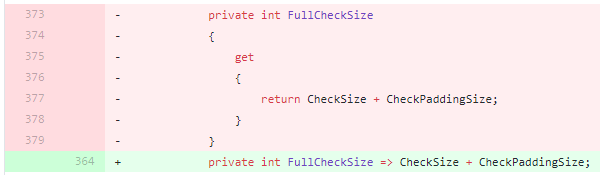
\includegraphics[width=0.7\textwidth]{getSetEx}
            \caption{A GitHub diff showing the change of a get block into a lambda expression in the Windows Forms repository.}
            \label{fig:getSetEx}
        \end{figure}

        The  next most common construct to be subject to change was the null-coalesce operator. Of the 133 changes, 65.4\% of the introductions of the null-coalesce operators were the expected `default' case: replacing an if-statement null-check. The remaining 34.6\% were only marginally different, replacing null-checks that used ternary if-statements over their regular counterparts. All of these changes were found in the C\# Winforms repo.

        Next in terms of frequency was null-conditional, in a similar manner to null-coalesce, replacing if-statements and/or ternary if-statements, as described above. Just like with null-coalesce too, all of these changes were found in the Winforms repo.

        Just behind that in number of occurrences is the use of compound assignment operators, with 37 instances of a change. All bar one of these instances was in the Winforms repo, with just a single replacement found in the Checkstyle repo. There was little scope for how these operators could replace other syntax, but by way of confirmation, all occurrences simply replaced two discrete operators with their compound equivalent. These operators are generally very common, but by convention in teaching courses from many programmers' formative years, they are introduced early on as a useful shorthand - it makes sense then that it's less likely for developers to need to go back over code and introduce these operators, as the chances are that they are already there.

        Ternary if-statements were next, being introduced over standard if-statements 20 times, all in the Winforms repo. In the Checkstyle repo, there was also one instance of a ternary if-statement being replaced with a regular if-statement.

        The second-least changed, foreach loops, has changes found across three repos, in all three languages present. 10 instances of a traditional for loop were replaced with a foreach loop, and 6 instances (in JavaScript) of a \codeword{forEach} function with a lambda being replaced by a \codeword{for-of} loop, one of a number of foreach-like looping structures available in JavaScript.

        Finally, no changes involving unary increment/decrement operators were identified at all in the any of the 22 commits. In the same manner as with compound operators, unary operators are often introduced as common shorthand that many programmers will use out of habit. In this case, we can surmise that either these operators were not wanted or required, or perhaps more likely, they were already in use in all places deemed necessary by the repo contributors.

    \subsection{Intermediate Language Comparison}
    \label{subsec:ilComp}
        To aid in confirming or denying some of the claims made in the survey by some participants, and to provide more general information about the constructs, the intermediate language code produced by the C\# and Java compilers was compared for both `plain' and `advanced' syntax.

        C\# was compiled using SharpLab and the Roslyn compiler from March 3\textsuperscript{rd} 2021. Java was compiled locally with JDK version 14.0.1 and the .class files were read by the JVM Bytecode Viewer extension for Visual Studio Code.

        The comparison will be broken down by construct and then detailed per language:

        \begin{itemize}
            \item In-line / Ternary If-statement
            \begin{itemize}
                \item \textbf{C\#} - Both versions are the same length, and both use two return statements (as is used in the plain source code). In the source code, the Boolean expression used is \codeword{temp < 20.0}: in the \emph{plain} IL, the logic for the condition is inverted, using a `branch if greater than or equal' instruction while the advanced IL uses a `branch if less than' instruction as would normally be assumed.
                \item \textbf{Java} - Plain follows the source code one-to-one, using two return instructions at the end of each code branch, whereas advanced uses a \codeword{goto} instruction on the true branch to jump to a single return instruction used by both code branches. This means that on one code branch, one additional instruction will be executed when using a ternary if-statement. In the same fashion is in C\#'s plain IL, both Java IL versions invert the Boolean logic and use a `branch if greater than or equal' instruction.
            \end{itemize}
            \item Lambda Expressions
            \begin{itemize}
                \item \textbf{C\#} - The lambda in the advanced version is much more complex in IL than in the source code: a kind of entire class is created to hold the actual method that is defined in line in source. This class has a public and private constructor and the desired method, generating 54 lines of code that are completely absent in the plain version. The method itself within this class is identical to that of the plain version. The actual code that \emph{calls} the lambda is only three instructions, compared to the plain version's six, however, this is also preceded by nine additional instructions that create and load an instance of the lambda's class. For such a small code snippet as is used here, it seems as though the potential overhead of a lambda may prove to have a negative impact. In the case of reuse however, this could change. This also goes further still to showing that lambdas are a deeper construct than they had were initially given credit for in the early stages of this study.
                \item \textbf{Java} - Very similar to C\# again, the in-place calling of the lambda is shorter than the plain equivalent, but there is additional code elsewhere in the file, effectively defining the lambda method as if it were a regular method (which is again the same length of the plain method). The inclusion of a lambda also adds 22 entries to the constant pool to help find the lambda method and call it at runtime. In Java, this boilerplate amounts to 43 additional lines in unedited bytecode.
            \end{itemize}
            \item Null-coalesce (C\# only)
            \begin{itemize}
                \item \textbf{C\#} - The plain version here is quite one-to-one with the source code, declaring two variables of type \codeword{Person} and assigning them within code branches as expected. In contrast, the advanced version only uses the stack, and does not declare any local variables. This does also have the side effect of requiring a bigger stack allocation to run the method, the advanced version requiring a size of eight to the plain version's requirement of one. This format is likely attributed to some degree of optimisation taking place by seeing that the variable in the condition is only null ever set to null in the method. This optimisation is potentially dependent on the context.
            \end{itemize}
            \item Null-conditional (C\# only)
            \begin{itemize}
                \item \textbf{C\#} - Similar to null-coalesce, the advanced version is shorter and declares no local variables, instead using only the stack. This may again be an example of contextual optimisation.
            \end{itemize}
            \item Unary Increment Operators
            \begin{itemize}
                \item \textbf{C\#} - Neither the plain nor advanced versions are mapped one-to-one in IL. The plain version uses two local variables for \codeword{y} and \codeword{z}, and \codeword{x} is maintained on the stack. In the advanced version, \codeword{x} and \codeword{y} are stored locally and \codeword{z} is maintained on the stack. Slightly different optimisation paths have been taken here producing slightly different code paths to the same result, the advanced version being two instructions longer. If all three variables used in this method were used more elsewhere, it is likely that all three would be stored in a local variable rather than one residing only on the stack.
                \item \textbf{Java} - The plain IL is a one-to-one mapping of the source code with no optimisation visible. However, the advanced IL makes use of a dedicated increment instruction, \codeword{iinc}, that directly maps to the \codeword{++} operator in the source code. This reduces the length of the IL by four instructions due to not needing to store the value back in the local variable as frequently.
            \end{itemize}
            \item Compound Assignment Operators
            \begin{itemize}
                \item \textbf{C\#} - No local variable is used, the value to print is maintained only on the stack for both advanced and plain, there is no difference between the plain and advanced in the IL.
                \item \textbf{Java} - Unlike in C\#, no optimisation is present for the plain IL, as it maps directly to the source code. In the advanced IL however, \codeword{iinc} is used to increment the value of a local variable by three (an argument to the IL instruction), cutting the instruction count by three.
            \end{itemize}
            \item Foreach Loops
            \begin{itemize}
                \item \textbf{C\#} - The plain IL is again effectively a one-to-one mapping of the for loop, albeit with the ordering of the three statements in the for loop signature moved to where they are actually executed. Array accessing in the plain version has been converted to a method call in the IL, as has the statement \codeword{nums.Count}. Similarly in the advanced version, the implicit use of an enumerator has been converted to explicit method calls. The advanced IL is eight lines longer, but both versions use the same number of external method calls within the loop itself. The advanced IL also requires a try-finally structure and an additional method call to dispose of the enumerator, used to iterate over the list, after the looping is complete.
                \item \textbf{Java} - Both versions are quite similar, sharing most normal instructions, but different external methods are called albeit that they are performing the same function (condition: \codeword{size()} vs. \codeword{hasNext()}, get element: \codeword{get()} vs. \codeword{next()}). The advanced IL does have an additional method call to get the iterator itself. Both are the same length in-place, but as with the lambda expression, this generated more code elsewhere, namely in the constant pool, adding 35 entries, compared to the regular for loop adding only 28.
            \end{itemize}
        \end{itemize}
\newpage
\section{Conclusion}
\label{sec:conclusion}
    This study has examined the ways and volumes in which seven different advanced programming language constructs (in three languages) are used by software developers and programmers. Upon seeing that there appears to be quite a lack of formal research into this topic, a survey was first carried out to collect information on how developers use these constructs and their thoughts on when and why the constructs should and shouldn't be used. Further, four open source repositories on GitHub were analysed first by static code analysis tools, and then manually by hand to find both what recommendations analysis tools do and don't give around the constructs, and to find the actual use these constructs in real production code. As a final comparison, the intermediate languages of C\# and Java were both compared to their source code for code that uses and doesn't use advanced constructs to learn if any of the constructs truly are `just' syntactic sugar and have no real effect on code in practice.
    
    This section will summarise the key findings from this study.

    \subsection{Findings}
        \subsubsection{Influences on Developers}
            It was assumed at the start of this study that developers were most influenced by style guides provided by their organisation that defined how their code should be stylised. However, only a small number of survey participants attributed this to their reasons for using most of the constructs. Ternary if-statements and lambdas certainly had a non-trivial number of selections for this reason, but code simplicity and clarity were the primary reasons selected. Some participants justified their motivations further in text, claiming that the main reason they style their code in any particular way was down to personal preference and their habits picked up during their early days programming and later throughout their careers. While only a minority of participants explicitly stated personal preference as a reason, via lack of other suggestions, it is reasonable to assume that many more developers rely on their own personal preference to lead their programming style.

            On the other side of the argument, the same principals applied: maintaining clarity was cited by nearly half of survey participants as the reason for them not to use any given construct, this being the most common reason for all seven constructs individually. Foreach loops were also marked out as possibly having a negative effect on the execution speed of code. This suggestion has not been tested formally in this study.

            In terms of performance, it was strongly indicated that participants thought that either there would be no change in performance, or they didn't know what effect there would be when using six of the seven constructs. Foreach loops were the one exception, with a greater proportion than other constructs indicating that they thought there would be decreased performance using a foreach loop.

            It was also discovered that there are some constructs that many developers will simply always use, namely foreach loops (some in spite of the performance implications), unary increment/decrement operators, and compound assignment operators.
            \\
            ISS were also unable to provide any company-wide coding style guidelines for reference in this study. I am led to believe that there \emph{are} guides that have been distributed to developers, but over years these have been remade, edited, amended, beyond a point where there is no longer one consistent style document for reference. This may have introduced a bias in the survey results regarding company style's influence on developers.
            \\

            A set of `sample' code files were written to contain examples of all the constructs, both in their plain syntax form, and the equivalent using the constructs. These files were bare skeleton code with no real function other than to provide a compilable source code file the contained all of the constructs. These were passed into static analysis tools SonarQube and Semgrep to find if any recommendations were made that could generally act as guidance to developers who run these tools against their code either as a one-off or as part of a CI/CD toolchain. Both tools reported next-to-nothing. The only relevant recommendation made was reported by SonarQube, recommending that a traditional for loop in JavaScript should be replaced by a \codeword{for-of} loop.

            It's difficult to criticise the analysis tools here, as it's likely that they are designed to work on code that has much more context, not in the relative isolation afforded in the sample files.

        \subsubsection{Construct Use in Real Code}
            The same static analysis tools as in the previous section were also used to process four open source GitHub repositories. Both tools were not able to be used to process all repos due to various technical and feature availability factors detailed earlier. Given the results of the combinations of tools and repos that did work, it is unlikely that any major recommendations were missed, as once again nearly no relevant issues were reported, and those that were reported are not of enough interest to repeat here.
            
            This lack of recommendations can lead us to one of two conclusions: the code in question has already been run through these tools or similar to address any issues, \textbf{or} these tools are not very effective at raising, or simply do not raise, issue with the constructs being examined here. Determining which of these two takes greater precedence would require further research.
            \\

            Manual analysis of the same code using more simplistic methods was able to provide much more insight into how the constructs are handled in real code. The focus was to identify any instances of syntax being swapped from plain syntax to construct or vice-versa. Excluding one commit (containing 441 instances of both a lambda and null-coalesce operator being added) as an outlier, the majority of changes (78\%) changed plain syntax to a construct. Of these, the most often changed was lambdas, specifically swapping out C\# \codeword{get {...}} and \codeword{set {...}} code blocks for lambda expressions instead.

            The data gathered from this is not hugely informative at a granular level unless examining the specifics of each repository, however, zooming out to see the larger picture, we can see that in general, these constructs are preferred over plain syntax. There are a minority (4.1\%) of occasions where the plain is preferred. As most of the changes (95.3\%) examined came from one repo, the WinForms repo, it's possible that these results may not generalise well to other codebases. However, as the WinForms repo, albeit open source, is maintained by Microsoft, one of the largest technology companies in play today, it stands to reason that they and their practices will be looked upon and used as exemplar in many situations. Through this, these results may be able to be generalised further than would normally be expected.

        \subsubsection{Effects of Constructs on Compiled Code}
            For C\# and Java, an intermediate language (IL) is generated in compilation, this IL is then interpreted at execution time on a per-platform basis. A certain level of optimisation takes place at both compile-time and runtime, but at compile-time we are able to interrogate the IL to find what, if any, optimisation was taken in the cases of plain syntax vs. the advanced constructs. For this analysis, modified versions of the previously mentioned sample code was compiled, the modification being to split the plain and advanced syntax methods each into their own files.

            As is often the case to the eyes of a layman when, looking at compiled code some oddities arose without explanation. For example, the inversion of some Boolean login statements (that didn't happen when using a ternary vs. a regular if-statement). Irrespective of use of syntax, it was found that C\# performed more optimisation at compile time than Java, the latter often mapping one-to-one to the source code. C\# was particularly clever with null-coalesce and null-conditional, doing away with local variables in favour of using the stack instead. Java also displayed a tangible change when using unary increment operators over the plain equivalent, as the Java Bytecode instruction set includes an explicit instruction to handle incrementing by any value. Whether or not this translates to an actual improvement at runtime would require more and extensive testing.

            Specific examples aside, none of the seven constructs were equal to their plain counterparts, all constructs generated different IL and are not the simple syntactic differences that some developers may consider them to be. Some differences are quite small (if-statement vs. ternary), but others create very different IL, requiring significant amounts of boilerplate and supporting code (lambdas and foreach loops). This begs the question: is there a tangible, measurable performance difference between using plain or advanced syntax? Is this difference, if present, variable on different execution platforms? This is outside the scope of this study but would be an interesting starting point for further study.

    \subsection{Review of Aims}
        The following list repeats the aims presented at the start of this report, with each aim followed by a description of how the aim was fulfilled.
        \begin{itemize}
            \item \textcolor{gray}{\textit{To understand the usage of seven advanced programming constructs.}}
                The survey showed many patterns in developers' use of constructs, including the notion of relying more on personal preference than solid resources. Manual analysis of the GitHub repositories also showed that, at times plain syntax is actively replaced by construct equivalents.
            \item \textcolor{gray}{\textit{To study what reasons developers have to, or to not, use these constructs.}}
                Developers' most commonly cited maintaining clarity and simplicity of code (according to their preference) as their primary influence in deciding how to style their code. Static code analysis tools also showed that they are somewhat unlikely to be able to provide much guidance to developers in this area.
            \item \textcolor{gray}{\textit{To research how these constructs are actually used in practice.}}
                The survey gave some insight into a few specific examples of when and where developers use certain constructs (e.g. some will always use unary increment operators) and the manual repository analysis also showed an array of unique instances of plain syntax being replaced with constructs. The most commonly seen was C\# \codeword{get} and \codeword{set} blocks being replaced by a lambda.
            \item \textcolor{gray}{\textit{To examine the effects of using these constructs has on compiled code.}}
                Examining the intermediate languages of C\# and Java showed that all of the constructs produce different IL to their plain syntax counterparts. It highlighted these differences and also showed the large amount of boilerplate code required for foreach loops and lambda expressions.
        \end{itemize}

    \subsection{Reflections}
        This section will briefly cover potential flaws and shortcoming within this study for future reference.

        \subsubsection{Lambdas}
        \label{subsubsec:lambdas}
            As has been referenced multiple times throughout this report, lambdas as a construct and language feature stood out from the rest of the constructs even in the first survey results. During the proceeds of this study it came to light that lambdas are a much more complex and powerful language feature than just that of a differing, more friendly, or more useful syntax structure. As mentioned by one participant in the survey results (see Section \ref{subsubsec:freeFormComments}), lambdas allow a programmer to use much more functional language programming practices that are not normally available in procedural and object-oriented languages like C\# and Java. In the same vein, in the survey results (see Section \ref{subsubsec:toUse}), it was noted that there are situations where a traditional method cannot be used in place of a lambda, and a lambda expression is the \emph{only} option.
            
            This was also hinted at further when examining the intermediate languages for both C\# and Java, as the inclusion of a lambda expression entailed the inclusion of a large amount of ancillary code, more so than would have been expected by a layman given the framing of the seven constructs together.
            
            The conclusion to draw from this is that lambdas should not have been grouped with the other constructs here; it is a much more powerful language feature, such that to assume it has the same side-effects, requirements, and use cases of the other constructs will cause confusion and other issues, as evidenced throughout.

        \subsubsection{Survey Wording}
        \label{subsubsec:surveyWording}
            There are a few questions in the survey which are not quite clear enough in what they mean. This particularly applies in the `to use' and `to not use' questions. Reference is made to making code `simpler' and/or `clearer', and conversely to making code `less clear' and/or `more complex'. These terms are somewhat vague and open to interpretation, the word `complex' is also potentially confusing, and it could have implied reference to the cyclic complexity of the code or otherwise caused confusion among respondents.

            Also in these two questions, while the options were open-end in a way (via providing the `None of these' option with a free-text box), there could have been, and likely should have been, a much richer selection of default options, such as options referencing online resources, books, colleagues, existing code, and so on.

        \subsubsection{GitHub Repository Selection}
            As was mentioned in Section \ref{subsubsec:osRepos}, the selection of GitHub repositories was intended to select the most popular repositories for each language, however, mistakenly, they were selected from the `trending today' list. Fortunately, these repositories were still large, well-maintained, and well-known repositories, but that was more by chance or accidental bias, than design due to this mistake.
        
        \subsubsection{Personal Reflections}
            Despite having written one dissertation of 10,000 words in my third year, this time round was no less daunting a task to see ahead. Finding a workable topic I found difficult at first, but after seeing the differing styles during my work for SCC.419, I decided to develop that further. Having done the research itself, the writing still appeared to be a near-insurmountable task, but the words tended to flow easily with there being so much to write about - even when this is only the second long-form essay I have written since A-levels.
            
            Analysing the survey data and the differences in the intermediate languages I found particularly interesting as many of my own assumptions were defeated, changed or extended in the process. I very much enjoy working into the low-level details in this way.

            I would have liked to have linked this closer to my work with ISS in SCC.419, but due to the nature of the work, there was little scope for such a link. Nevertheless, I was able to enhance this study by working with ISS and their developers as much as the final study design permitted.

    \subsection{Negative Impacting Circumstances}
        The on-going coronavirus pandemic is still very much a factor in the lives us all, and this has been no different for me during the entire timeline of this study and dissertation. Much like many others, I have been relatively confined to one-room student accommodation for the duration of this academic year as restrictions have loosened and tightened on and off over time. While far from the worst-affected, this has still had a marked effect on both my mental and physical health, and also my general productivity throughout.
        
    \subsection{Future Research}
        Due to the apparent relative lack of formal research into this area, there is great potential for further research. In essence, these points can be distilled into repeating many of the study parts here, but over a larger/better sample set, now that it has been found that there maybe information of interest in such a topic.
        
        Firstly, a similar survey (with issues noted in Section \ref{subsubsec:surveyWording} addressed) may be carried out over a much large population, using a much more generalisable sample of developers. This could help further understanding of the motivation behind programmers' use of certain language syntax and structures.
            
        If more time and resources are available, a greater number of static code analysis tools, including paid-for tools could be employed, or further still, dynamic/runtime analysis or profiling tools could be used to discover if any recommendations or issues are raised by these tools. Given the small amount of data gathered from such tools in this study though, this may not be particularly high priority.
        
        With significantly more time, a greater number of large GitHub codebases could be hand-analysed for every use of the constructs detailed in this study, perhaps to learn how much committed code uses such constructs from the first moment it is pushed or to otherwise more exhaustively check the use of the constructs in the same way carried out here.
            
        Finally, and perhaps most interestingly, in terms of providing hard data, accurate and fine-grained software profiling and benchmarking may be undertaken on sample code files as in this study to measure if there is a tangible effect on performance that comes from using any or all of these constructs. A deeper study could attempt to strip out all uses of a construct from an application (or to replace all plain syntax with a construct version) and to then measure its performance to see then, in context, if the constructs have a measurable effect on performance.
    
    \subsection{Closing Statement}
        This goal of this study was somewhat vague in the very early stages of planning, and over time it became clear this was to be a very exploratory study over anything else. Hopefully this should prove to be one of the early steps in research into the practice of programming from a new meta-perspective. Further research could help lead to a better understanding of how we as programmers write code, which may then give rise to knowledge that, if discussed enough,  will aid software industry to clear up uncertainty and perhaps, if only slightly, unify coding style and programming practices.

\newpage
\bibliography{ref}
\newpage
\section*{Appendix}
    \includepdf[scale=0.8, pages=-, pagecommand=\subsection*{A: Survey}]{../Ref/survey}
    \includepdf[scale=0.8, pages=-, pagecommand=\subsection*{B.1: Sample C\# Source Code File}]{../Ref/SampleCS}
    \includepdf[scale=0.8, pages=-, pagecommand=\subsection*{B.2: Sample JavaScript Source Code File}]{../Ref/SampleJava}
    \includepdf[scale=0.8, pages=-, pagecommand=\subsection*{B.3: Sample Java Source Code File}]{../Ref/SampleJS}
    \includepdf[scale=0.8, pages=-, pagecommand=\subsection*{C: Project Proposal}]{../Ref/proposal}

\end{document}